\begin{filecontents*}{example.eps}
%!PS-Adobe-3.0 EPSF-3.0
%%BoundingBox: 19 19 221 221
%%CreationDate: Mon Sep 29 1997
%%Creator: programmed by hand (JK)
%%EndComments
gsave
newpath
  20 20 moveto
  20 220 lineto
  220 220 lineto
  220 20 lineto
closepath
2 setlinewidth
gsave
  .4 setgray fill
grestore
stroke
grestore
\end{filecontents*}
%\documentclass{svjour3}                     % onecolumn (standard format)
\RequirePackage{fix-cm}
%
%\documentclass{svjour3}                     % onecolumn (standard format)
%\documentclass[smallcondensed]{svjour3}     % onecolumn (ditto)
%\documentclass[smallextended]{svjour3}       % onecolumn (second format)
\documentclass[twocolumn]{svjour3}          % twocolumn
%
\smartqed  % flush right qed marks, e.g. at end of proof
%
\usepackage{appendix}
\usepackage{amsmath}
\usepackage{graphicx}
\usepackage[switch]{lineno}
\usepackage{array}
\usepackage{longtable}
\usepackage{natbib}
\usepackage{hyphenat}
\bibliographystyle{ieeetr}
\setcitestyle{square}
\setcitestyle{citesep={,}}


\linenumbers

\newcommand*\patchAmsMathEnvironmentForLineno[1]{%
\expandafter\let\csname old#1\expandafter\endcsname\csname #1\endcsname
\expandafter\let\csname oldend#1\expandafter\endcsname\csname end#1\endcsname
\renewenvironment{#1}%
{\linenomath\csname old#1\endcsname}%
{\csname oldend#1\endcsname\endlinenomath}}% 
\newcommand*\patchBothAmsMathEnvironmentsForLineno[1]{%
\patchAmsMathEnvironmentForLineno{#1}%
\patchAmsMathEnvironmentForLineno{#1*}}%
\AtBeginDocument{%
\patchBothAmsMathEnvironmentsForLineno{equation}%
\patchBothAmsMathEnvironmentsForLineno{align}%
\patchBothAmsMathEnvironmentsForLineno{flalign}%
\patchBothAmsMathEnvironmentsForLineno{alignat}%
\patchBothAmsMathEnvironmentsForLineno{gather}%
\patchBothAmsMathEnvironmentsForLineno{multline}%
}


%\documentclass[catalysts,article,submit,moreauthors,pdftex,10pt,a4paper]{mdpi} 
\usepackage{todonotes}
\usepackage{comment}
\usepackage{graphicx}
%--------------------
% Class Options:
%--------------------
% journal
%----------
% Choose between the following MDPI journals:
% actuators, admsci, aerospace, agriculture, agronomy, algorithms, animals, antibiotics, antibodies, antioxidants, applsci, arts, atmosphere, atoms, axioms, batteries, behavsci, beverages, bioengineering, biology, biomedicines, biomimetics, biomolecules, biosensors, brainsci, buildings, carbon, cancers, catalysts, cells, challenges, chemosensors, children, chromatography, climate, coatings, computation, computers, condensedmatter, cosmetics, cryptography, crystals, data, dentistry, designs, diagnostics, diseases, diversity, econometrics, economies, education, electronics, energies, entropy, environments, epigenomes, fermentation, fibers, fishes, fluids, foods, forests, futureinternet, galaxies, games, gels, genealogy, genes, geosciences, geriatrics, healthcare, horticulturae, humanities, hydrology, informatics, information, infrastructures, inorganics, insects, instruments, ijerph, ijfs, ijms, ijgi, inventions, jcdd, jcm, jdb, jfb, jfmk, jimaging, jof, jintelligence, jlpea, jmse, jpm, jrfm, jsan, land, languages, laws, life, literature, lubricants, machines, magnetochemistry, marinedrugs, materials, mathematics, mca, mti, medsci, medicines, membranes, metabolites, metals, microarrays, micromachines, microorganisms, minerals, molbank, molecules, mps, nanomaterials, ncrna, neonatalscreening, nutrients, particles, pathogens, pharmaceuticals, pharmaceutics, pharmacy, philosophies, photonics, plants, polymers, processes, proteomes, publications, recycling, religions, remotesensing, resources, risks, robotics, safety, sensors, separations, sexes, sinusitis, socsci, societies, soils, sports, standards, sustainability, symmetry, systems, technologies, toxics, toxins, universe, urbansci, vaccines, vetsci, viruses, water
%---------
% article
%---------
% The default type of manuscript is article, but can be replaced by: 
% addendum, article, book, bookreview, briefreport, casereport, changes, comment, commentary, communication, conceptpaper, correction, conferencereport, expressionofconcern, meetingreport, creative, datadescriptor, discussion, editorial, essay, erratum, hypothesis, interestingimage, letter, newbookreceived, opinion, obituary, projectreport, reply, retraction, review, sciprints, shortnote, supfile, technicalnote
% supfile = supplementary materials
%----------
% submit
%----------
% The class option "submit" will be changed to "accept" by the Editorial Office when the paper is accepted. This will only make changes to the frontpage (e.g. the logo of the journal will get visible), the headings, and the copyright information. Also, line numbering will be removed. Journal info and pagination for accepted papers will also be assigned by the Editorial Office.
%------------------
% moreauthors
%------------------
% If there is only one author the class option oneauthor should be used. Otherwise use the class option moreauthors.
%---------
% pdftex
%---------
% The option pdftex is for use with pdfLaTeX. If eps figure are used, remove the option pdftex and use LaTeX and dvi2pdf.

%=================================================================

%------------------------------------------------------------------
% The following line should be uncommented if the LaTeX file is uploaded to arXiv.org
%\pdfoutput=1

%=================================================================
% Add packages and commands here. The following packages are loaded in our class file: fontenc, calc, indentfirst, fancyhdr, graphicx, lastpage, ifthen, lineno, float, amsmath, setspace, enumitem, mathpazo, booktabs, titlesec, etoolbox, amsthm, hyphenat, natbib, hyperref, footmisc, geometry, caption, url, mdframed

%=================================================================
%% Please use the following mathematics environments:

%% For proofs, please use the proof environment (the amsthm package is loaded by the MDPI class).
\makeatletter
%\def\@biblabel#1{}
%\renewenvironment{thebibliography}[1]
%     {\section*{\refname}%
%      \@mkboth{\MakeUppercase\refname}{\MakeUppercase\refname}%
%      \list{\@biblabel{\@arabic\c@enumiv}}%
%           {\settowidth\labelwidth{\@biblabel#1{}}%
%            \leftmargin\labelwidth
%            \advance\leftmargin16pt
%            \advance\leftmargin\labelsep
%            \setlength\itemindent{-16pt}
%            \@openbib@code
%            \usecounter{enumiv}%
%            \let\p@enumiv\@empty
%            \renewcommand\theenumiv{\@arabic\c@enumiv}}%
%      \sloppy
%      \clubpenalty4000
%      \@clubpenalty \clubpenalty
%      \widowpenalty4000%
%      \sfcode`\.\@m}
%     {\def\@noitemerr
%       {\@latex@warning{Empty `thebibliography' environment}}%
%      \endlist}
%\renewcommand\newblock{\hskip .11em\@plus.33em\@minus.07em}
\makeatother

\makeatletter
%\renewcommand{\@biblabel}[1]{{}\hfill}
\makeatother
%=================================================================
% Full title of the paper (Capitalized)
\title{Transition-Metal Dopants in TiO$_2$ for Photocatalytic Nitrogen Fixation}

% Authors, for the paper (add full first names)

\author{Benjamin M. Comer$^{1 \dagger}$, Max H. Lenk$^{2}^{\dagger}$, Aradhya P. Rajanala$^{3}$, Emma L. Flynn$^{4}$, Andrew J. Medford$^{1}$*}
% Authors, for metadata in PDF

% Affiliations / Addresses (Add [1] after \address if there is only one affiliation.)
%\address{
%$^{1}$ \quad School of Chemical and Biomolecular Engineering, Georgia Institute of Technology\\
%$^{2}$ \quad School of Materials Science and Engineering, Georgia Institute of Technology\\
%$^{3}$ \quad School of Physics, Georgia Institute of Technology\\
%$^{4}$ \quad School of Computer Science, Georgia Institute of Technology\\
%}

% Contact information of the corresponding author
%\corres{Correspondence: ajm@gatech.edu}

% Current address and/or shared authorship
%\firstnote{Current address: Affiliation 3} 
%\firstnote{These authors contributed equally to this work.}

\institute{
$^{1}$ School of Chemical and Biomolecular Engineering, Georgia Institute of Technology\\
$^{2}$ School of Materials Science and Engineering, Georgia Institute of Technology\\
$^{3}$ School of Physics, Georgia Institute of Technology\\
$^{4}$ School of Computer Science, Georgia Institute of Technology\\
$\dagger$ These authors contributed equally to this work. \\
* Correspondence \email{andrew.medford@chbe.gatech.edu}\\
  311 Ferst Drive NW, Atlanta, Georgia 30318 \\
  Tel.:+1 (404) 385-5531\\
           %  \\
%             \emph{Present address:} of F. Author  %  if needed
}
\authorrunning{B. Comer et. al.}
% Simple summary
%\simplesumm{}

% Abstract (Do not use inserted blank lines, i.e. \\) 


% Keywords
%\keyword{ammonia synthesis; single atom catalysis; \textit{d}-band model; density functional theory}

% The fields PACS, MSC, and JEL may be left empty or commented out if not applicable
%\PACS{J0101}
%\MSC{}
%\JEL{}

% If this is an expanded version of a conference paper, please cite it here: enter the full citation of your conference paper, and add $^\S$ in the end of the title of this article.
%\conference{}

%%%%%%%%%%%%%%%%%%%%%%%%%%%%%%%%%%%%%%%%%%
% Only for the journal Data:

%\dataset{DOI number or link to the deposited data set in cases where the data set is published or set to be published separately. If the data set is submitted and will be published as a supplement to this paper in the journal Data, this field will be filled by the editors of the journal. In this case, please make sure to submit the data set as a supplement when entering your manuscript into our manuscript editorial system.}

%\datasetlicense{license under which the data set is made available (CC0, CC-BY, CC-BY-SA, CC-BY-NC, etc.)}

%%%%%%%%%%%%%%%%%%%%%%%%%%%%%%%%%%%%%%%%%%
\begin{document}


\maketitle
\begin{abstract}

%Developing novel, carbon-neutral methods of generating fixed nitrogen for chemicals and fertilizers is a vital step toward decarbonizing the global economy. TiO$_2$ has been observed to fix nitrogen at ambient pressure under illumination using only humidity and air. However, rates for this reaction remain low over a half-century after the discovery of the process. In this work, we investigate the use of surface metal dopants to promote surface reactions by altering the thermodynamics of intermediates on the rutile TiO$_2$ (110) surface. We screen all d-block transition metal dopants for stability and promotion of the reduction of nitrogen to ammonia. We find that the formation energy of surface metal dopant sites follows a trend described by the \textit{d}-band model, with sites becoming more stable from left to right on the periodic table. The binding energies of N$_2$, N$_2$H, and NH$_2$ all reach maximums on metal sites in the middle of the d-block. These energies trend with the cohesive energy as calculated by the Friedel model. The adsorption energies of intermediate species are correlated with each other and the \textit{d}-band center, suggesting that the \textit{d}-band model holds for single metal atoms doped into oxide surfaces. The catalytic activity of the metal-doped systems shows a volcano type relationship with the NH$_2$ binding energy as a descriptor. The metals predicted to be most active are Rh, Tc, and Co, but their activity is predicted to be comparable to that of Ti, indicating that metal-doped surface sites likely do not contribute significantly to photocatalytic nitrogen reduction.

%%%%%%%% catalysis letters requests an approximately 50 word abstract. I see others with ~150 word abstracts, so let's aim for that

In this work, we screen all d-block transition metal dopants for surface site stability and promotion of the reduction of nitrogen to ammonia on TiO$_2$. We find a linear relationship between \textit{d}-band center and dopant site formation energy. The binding energies of N$_2$, N$_2$H, and NH$_2$ all are strongly correlated with the cohesive energies of the dopant metals, reaching maximums on metal sites in the middle of the d-block. The activity of the metal-doped systems shows a volcano type relationship with the NH$_2$ energy as a descriptor.

\end{abstract}
\section{Introduction}
%%boilerplate Haber-Bosch intro
The fixation of atmospheric nitrogen has long been one of the prime challenges in chemistry and chemical engineering \cite{ritter_18, Schloegl_2003}. The Haber-Bosch process has been the route of choice for performing nitrogen fixation for the past century, permitting much of the population growth over the last century \cite{Smil_1999}. However, this process has significant drawbacks, including high CO$_2$ emissions and centralized production due to large capital requirements \cite{Comer_2019}. The Haber-Bosch process's considerable contribution to CO$_2$ emissions has been an increasingly pressing concern for the global community, as it accounts for 340 million tonnes of CO$_2$---fully 2\% of the carbon emissions worldwide \cite{gross_12, Schiffer_2017}. For this reason, supplanting the Haber-Bosch process would represent a significant contribution to global efforts to curb climate change. Another drawback lies in the centralization of the Haber-Bosch process, which leads to high transportation costs and contributes to global economic inequality \cite{Comer_2019}.  Due to the high pressures and pure feedstocks required, Haber-Bosch has significant economies of scale. Constructing a new plant requires significant capital and natural resources, as well as a critical mass of demand. Industrialized nations meet these criteria through a constant availability of capital and industrialized agricultural with a steady demand for fertilizer \cite{McArthur_2017}. However, these barriers have prevented developing regions, such as Sub-Saharan Africa, from developing Haber-Bosch plants. The lack of local production results in high costs of fertilizers due to transportation, corresponding to reduced crop yields, which lowers demand and further increases prices. \cite{IFDC_2012} This causes the fertilizer to be most expensive in regions where it is most needed.

Due to the various drawbacks of the Haber-Bosch process, researchers have sought alternative means of producing fixed nitrogen \cite{Comer_2019, McPherson_2019, WANG20181055, Kyriakou_2017, de_Bruijn_2015, Michalsky_2015}. 
%These methods typically focus on optimizing catalyst structure under different conditions but also extend to techniques such as genetically engineering crops to harbor nitrogen fixing bacteria \cite{de_Bruijn_2015}. Another technique is chemical looping, a process in which a metal hydride hydrogenates nitrogen and releases it through oxidation of the metal. The metal is subsequently hydrogenated \cite{Michalsky_2015} to achieve a closed chemical cycle. Chemical looping suffers from the high temperatures required for the metal rehydrogenation. 
Two strategies that have received significant recent interest are electrocatalysis \cite{McPherson_2019} and photocatalysis \cite{Medford_2017}. However, making either of these technologies viable presents a significant challenge. Electrochemical nitrogen fixation requires generating electricity and transporting electrons to the catalyst surface to perform the reaction \cite{Kyriakou_2017}. The need for both solar and electrocatalytic cells may limit the viability of electrochemical processes in the developing world \cite{Comer_2019}. An alternative route is photochemical nitrogen fixation, where the catalyst is placed in direct contact with sunlight, air, and water vapor  to produce fixed nitrogen. The photochemical route has the potential to operate with low capital investment and simpler infrastructure, making it promising for low-resource environments.

%review photocatalytic nitrogen fixation experiments, then a paragraph on metal/nonmetal doping
The scientific community has known of photochemical nitrogen fixation for decades, but inconsistent results and low rates have discouraged further study \cite{Medford_2017}. N. Dhar \cite{Dhar_1941} was the first to investigate photocatalytic nitrogen, and the first well\hyp{}controlled experiments were performed decades later when Schrauzer and Guth independently re-discovered the process \cite{Schrauzer_1977}. Schrauzer and Guth were able to establish the production of NH$_3$ in sterilized desert sands under illumination, \cite{Schrauzer_1977} including confirmation via isotopic labeling \cite{Schrauzer_1983}. Numerous independent experiments have been performed over the years and reported photochemical production of NH$_3$ over titania materials \cite{Bickley_1979,Augugliaro_1982,Soria_1991,Li_2018,Yuan_2013,Hirakawa_2017}, though legitimate skepticism has remained due to issues with contamination \cite{edwards1992opinion, Davies1995, davies1993reply}, interference \cite{Gao_2018,Cui2018}, and inconsistent results \cite{Medford_2017}. However, recent experiments utilizing ambient pressure X\hyp{}ray Photoelectron Spectroscopy (AP\hyp{}XPS) have observed reduced nitrogen compounds under only under illumination \cite{Comer_2018b}. These experiments provide direct experimental evidence that photo\hyp{}induced nitrogen reduction occurs on titania surfaces, though the presence of carbon-based impurities was found to be a critical enabler of the process. %Indeed, it has proven critical to ensure great care is taken in NH$_3$ measurement methods, due to the low concentrations and interference of other species.\cite{Gao_2018,Cui2018}
%describe difference between photochemical and electrochemical systems

%discuss efficiency
Despite improved understanding of photocatalytic nitrogen fixation, the rates of reaction on titania-based catalysts remain relatively low ($\mu mol$ scale \cite{Hirakawa_2017}). The competition of NH$_3$ production with H$_2$ evolution is a key issue for electrocatalytic or photocatalytic nitrogen fixation and has been dubbed the ``selectivity challenge'' \cite{Singh_2017}. For this reason, high Faradic efficiency is also often sought in the electrochemical literature \cite{McPherson_2019}. The driver of this is the opportunity cost of using electricity for catalysis over other possible uses. For this reason, many electrochemical studies focus on low-overpotentials where the selectivity is generally highest, but the overall reaction rate is relatively low.

In contrast, photo-excited electrons are difficult to harvest for alternate uses, and hence the overall solar-to-ammonia efficiency is the key metric for assessing photocatalytic ammonia production. Rates on the order of 0.02\% solar-to-ammonia efficiency have been reported for pure titania catalysts \cite{Hirakawa_2017}. These rates are orders of magnitude lower than the $\sim$20\% solar-to-hydrogen efficiency achieved by state-of-the-art catalytic systems for solar hydrogen production \cite{Nakamura_2015, Jia_2016}. However, it has been posited that a comparatively low solar efficiency of $\sim$0.1-1\% may be sufficient to enable solar fertilizer technology \cite{Comer_2019, Medford_2017}. With sufficiently low capital cost, this system could see use in areas that are far from fertilizer plants due to the lowering of transportation costs. Thus, strategies for enhancing the rate of photocatalytic ammonia production on titania catalysts may be a viable route for designing nitrogen fixation catalysts.

One route to increasing reaction rates is the inclusion of transition\hyp{}metal dopants in TiO$_2$ \cite{Zaleska_2008}.  Transition\hyp{}metal dopants can increase rates via at least two distinct mechanisms: increasing the amount of photo-generated electrons that reach the surface by improving absorption and charge separation, or by altering the kinetics of the surface reaction.
%Doping metals within a semi-conductor can improve reaction rates by either altering the kinetics of the surface reaction or improving the material's photochemical properties of the material, such means as decreasing the band gap and tuning band alignment. 
Transition-metal doping has been previously explored to improve the performance of TiO$_2$ photocatalysts \cite{Schneider_2014, Li_2007, Dozzi_2013}. In particular, early work on photocatalytic nitrogen fixation tested a variety of metal dopants. These studies found that several noble metals \cite{Ranjit_1996} and iron in particular increase yields \cite{Schrauzer_1977, Schrauzer_1983, Augugliaro_1982, Soria_1991, Ranjit_1996, Ranjit_1997}. More recently, Hirakawa et al. found that depositing noble metals (Ru, Pt, Pd) onto an already prepared rutile (110) surface led to a decrease in reaction rates.\cite{Hirakawa_2017} This decrease in rates, along with detailed experimental and theoretical studies on the role of iron dopants  \cite{Soria_1991, Comer_2018} suggests that the primary mechanism of these previously-reported dopants is enhanced charge separation. However, transition-metal dopants are also known to affect the surface properties in a range of other materials and reactions \cite{Khan_2018, Gu_2014, Ammal_2016, Gu_2017, Comer_2018, Garc_a_Mota_2011, Yao_2017}. In particular, the field of ``single-atom catalysis'' has revealed that isolated transition-metal sites supported on oxide materials can exhibit remarkable catalytic properties \cite{Liu_2016, Qiao_2011, O_Connor_2018}. However, relatively little effort has been focused on understanding how isolated transition-metal atom dopants affect the surface reactivity of oxides for the conversion of nitrogen to ammonia \cite{Tao_2019, Liu_2019, Zhao_2019, Cheng_2019, Li_2017}.

%While much is known about the ability of dopant metals to change the bulk properties of a semiconducting material, however, photochemists rarely consider how doped metals at the surface could affect reaction kinetics. There is a sizable literature on the effects of metal sites in 2D materials\cite{Khan_2018}, and single atoms on oxide supports\cite{Liu_2016} and doped metal oxides \cite{Gu_2014, Ammal_2016 Gu_2017,Comer_2018, Garc_a_Mota_2011, Yao_2017}. This work focuses on doped metal oxide materials. 

%review theoretical work

%To expedite the process, avoiding a multitude of experimental tests on the domain of possible dopants, there have been attempts to predict catalytic activity computationally. Computational screening has been used profitably in several areas of catalysis including CO$_2$ reduction\cite{}, hydrogen evolution\cite{}, and oxygen reduction\cite{Norskov_004}. These theoretical studies screening materials for effectiveness in nitrogen fixation have confirmed its applicability as a predictive method.\cite{Hoskuldsson_2017} Theoretical results verify that the N$_2$ bond dissociation is the rate-limiting step. \cite{https://pubs.acs.org/doi/pdf/10.1021/jp056982h} Further endeavors focus on determining specific reaction pathways or finding more efficient ceramics, surfaces, and dopants.\cite{}
%describe challenges of ambient temperature N2 fixation

%The two largest challenges to fixing nitrogen under ambient conditions have been posited to be the kinetics of the first hydrogenation step and the desorption of NH$_3$ starting from NH$_2$.\cite{Hoskuldsson_2017,Singh_2017,Montoya_2015} These two challenges provide the basis of two design criteria for nitrogen fixation catalysts. N$_2$ is a molecules with no intrinsic dipole and a very strong N-N triple bond making reactions challenging at room temperature.\cite{Montoya_2015, Comer_2018}. This is the primary reason the first hydrogenation step is found to be rate limiting for low temperature nitrogen reduction.\cite{Montoya_2015, Singh_2017, Hoskuldsson_2017, Comer_2018} 
%The exceedingly high temperatures of the Haber-Bosch process (700K) allow it to follow a "dissociative" mechanism, whereby N$_2$ is dissociated on the catalyst surface into nitrogen adatoms immediately in the first step \cite{Ullmann_amm_2006, Hellman_2006}. Surmounting such a high energy barrier is not feasible at room temperature, requiring the reaction to follow an "associative" mechanism in which hydrogen atoms are attached successively to the nitrogen until the N-N bond can be broken.\cite{Montoya_2015} However, in cases where  NH$_x$ species tend to bind strongly to surfaces, making desorption of NH$_x$ species into the product NH$_3$ rate limiting. In the literature, the reaction from adsorbed NH$_2$* to fully desorbed NH$_3$ has been identified as rate limiting on catalysts with lower barrier for the first hydrogenation \cite{Hoskuldsson_2017}.

% review what we did in this publication then lead into results
In this work, we focus on the potential of isolated transition-metal atoms substituted into the rutile (110) titania surface as a potential route to improve the surface kinetics of the nitrogen reduction reaction. We screen The \textit{d}-block transition metals substituted onto the (110) surface in two different configurations corresponding to formal oxidation states of 2+ and 4+. 
%The 4+ slabs were generated by replacing the coordinatively unsaturated Ti with the studied metal. 2+ slabs were generated by substituting a six-fold Ti with the substituent metal and adding an oxygen vacancy at the bridging oxygen site such (see Figure \ref{fig:ex_slab}). 
We analyze the trends present across the periodic table with for the dopant formation energy, N$_2$ adsorption energy, N$_2$H, and NH$_2$ adsorption energy. We also map out the thermodynamics of all N$_2$ reduction pathways and use this to assess the most favorable reaction mechanism. Finally, we assess the expected improvement in reaction rates from forming metal dopant sites on the surface for photocatalytic N$_2$ reduction. The results illustrate that there are clear correlations in the formation and adsorption energies with the \textit{d}-band center and cohesive energies. These scaling relations resulting in an optimum in the rate-limiting potential for nitrogen reduction as a function of N$_2$H and NH$_2$ adsorption energies. %However, the optimum dopants are not predicted to be significantly more active than pure TiO$_2$, suggesting that transition-metal doping is not a good strategy for tuning the reactivity for photocatalytic ammonia fixation on titania. Nonetheless, the strong trends observed indicate that the \textit{d}-band center is a good descriptor of reactivity for metal dopants on titania. This correlation suggests that the \textit{d}-band model is a promising approach for selecting metal dopants in other oxide systems or designing single-atom catalysts supported on oxide materials.

\section{Results and Discussion}

Rutile TiO$_2$ (110) was chosen as a model surface based on the experimentally observed correlation between rutile content and reaction rates for photocatalytic nitrogen fixation\cite{Schrauzer_1977}. Additionally, there is a rich literature on the surface science of rutile (110) \cite{Diebold_2003, Yates_1991, Lu1994, Walle2009}, and recent surface-science experiments and DFT calculations indicate that carbon substitution defects on the rutile (110) surface are active for photocatalytic nitrogen reduction \cite{Comer_2018b}. From this model surface, slabs containing metal dopants at the surface in the 2+ and 4+ oxidation states were generated for each dopant metal (see Section \ref{sec:methods} for full details).
%The 2+ oxidation state was chosen, as all transition metals are able to hold a 2+ oxidation state\cite{Greenwood_chemistry_text_book}, allowing trends to be seen across the periodic table. The stability of metal dopants in the 4+ oxidation states were also investigated, and found to be more stable in general(see Figure \ref{fig:d_band}). 
In total, all d-block transition-metals, except Mn and Cr (23 total), were screened for their surface formation energy and activity for nitrogen reduction.  The binding energies of N$_2$H and NH$_2$ have been identified as descriptors for activity in the literature as they are typically involved in the rate-limiting steps \cite{Hoskuldsson_2017, Montoya_2015, Comer_2018}. Thus, these energies have been calculated to asses the activity of generated surfaces.  Full details of the calculation methodology are in the Methods section (Sec. \ref{sec:methods}).

%by mapping out the thermodynamics of all possible nitrogen reduction pathways on the surface. 

\begin{figure}
    \centering
    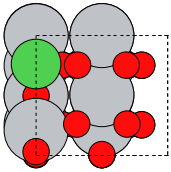
\includegraphics[width=0.5\linewidth]{Images/ex_2+_slab.png}
    %\caption{An example of the screened 2+ slabs. The substituent metal has replaced a 6 fold Ti atom (seen in blue) and a bridging oxygen vacancy has been formed to allow the metal to enter the 2+ oxidation state.}
    \label{fig:2+_ex_slab}
%\end{figure}

%\begin{figure}
    \centering
    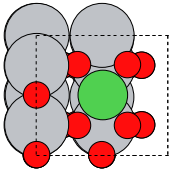
\includegraphics[width=0.5\linewidth]{Images/ex_4+_slab.png}
    \caption{An example of the screened 2+ (top) and 4+ (bottom) slabs. For 2+ sites the substituent metal has replaced a 6 fold Ti atom (seen in blue) and a bridging oxygen vacancy has been formed to allow the metal to enter the 2+ oxidation state.  For 4+ sites the substituent metal has replaced a five-fold Ti atom (seen in blue) resulting in a 4+ formal oxidation state.}%, and a bridging oxygen vacancy has been formed to allow the metal to enter the 4+ oxidation state.}
    \label{fig:2+ex_slab}
\end{figure}

%\subsection{Trends Across The Periodic Table}

%Studying the formation energy of 2+ metal substituted active sites and the binding energies of nitrogen species has revealed trends across the periodic table. The nature of these trends is based in electronic interactions between the metals' \textit{d}-band elections and the surface and adsorbates, as is commonly seen in catalysis \cite{Hammer_2000,Nilsson_2008, Greeley_2002}. However, full analysis of the electronic structures of these active sites is beyond the scope of this work, which focuses on the practical implications of the trends on catalytic systems.

\subsection{Trends In Active Site Formation Energies}

The stability of substituted metal surface sites was examined with respect to the position of their \textit{d}-band center. In Figure \ref{fig:d_band}a, the formation energy of the studied active sites has been plotted against the location of the \textit{d}-band center of the corresponding transition metal. The pure metallic form is the reference for the formation energy of each metal substituted site. The \textit{d}-band centers are also calculated from the metallic bulk state rather than the single atom. The plot indicates there is a strong correlation between the \textit{d}-band center and formation energy of the metal substitution (R$^2$ = 0.89). We can rationalize the observed correlation in the context of the \textit{d}-band model of chemical bonding \cite{Hammer_1995, Nilsson_2008} summarized in Equation \ref{eq:d_band} below:
%\onecolumn
\begin{figure*}
    \centering
    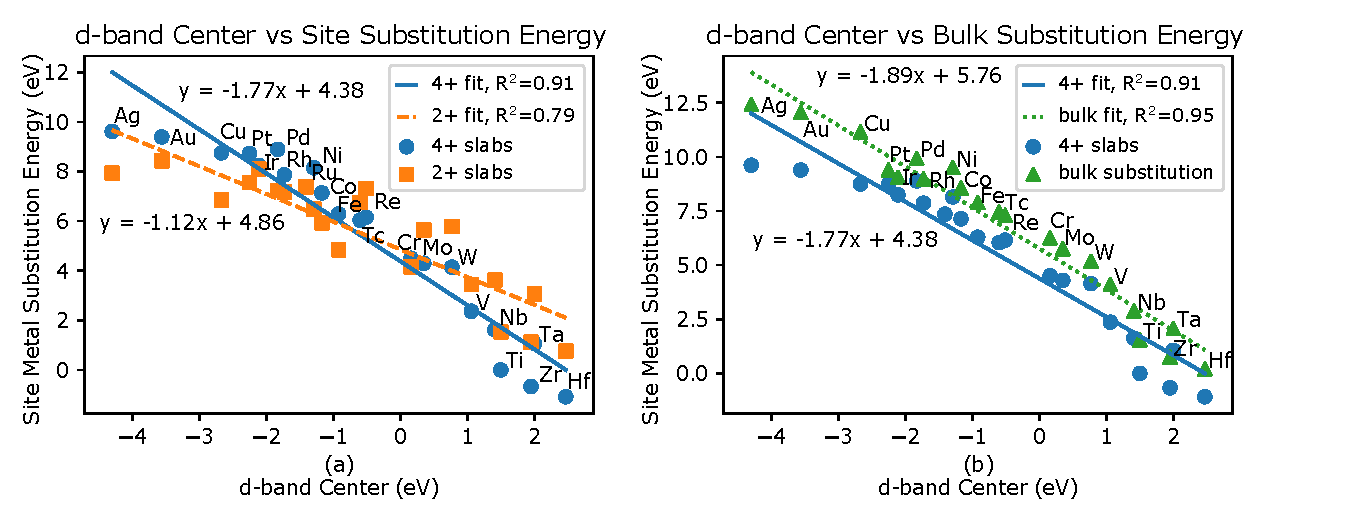
\includegraphics[width=0.9\linewidth]{Images/d_band_vs_formation.pdf}
    \caption{(a) The formation energy of 4+ surface sites (blue) and 2+ surface sites (orange) with respect to their bulk metallic state vs. the metallic \textit{d}-band center (b) The formation energy of 4+ surface sites (blue) and bulk substitutions (green) with respect to their bulk metallic state vs. the metallic \textit{d}-band center. \textit{d}-band centers were obtained from Ref. \citenum{Ruban_1997}. Only metals whose \textit{d}-band center was previously reported in Ref. \citenum{Ruban_1997} are included.}
    \label{fig:d_band}
\end{figure*}
%\twocolumn

\begin{equation}
    %E_{coh} = \epsilon_d + \epsilon_s \\
    \Delta E_d = \int^{E_F} E(\rho'(E) - \rho(E))dE
    \label{eq:d_band}
\end{equation}
where $\Delta E_d$ is the binding energy associated with interaction with the \textit{d}-band, $E_F$ is the Fermi level energy, $\rho(E)$ is the \textit{d}-band density of states before adsorption, and $\rho'(E)$ is the density of states after adsorption. The interaction between adsorbates and the metal's \textit{s}-states are assumed to be approximately constant for all metals, such that variations in binding energies are controlled primarily through bonding interactions with the \textit{d}-band. Interaction with the \textit{d}-band causes the orbitals of the adsorbate to separate into bonding and anti-bonding orbitals. As the \textit{d}-band center approaches the Fermi-level, the anti-bonding orbitals increasingly fill, leading to a weaker bond.

Our system involves a metal atom interacting with an oxide surface rather than an adsorbate binding to the metal surface. We hypothesize that the \textit{d}-orbitals of the integrated metal atom interact with the \textit{p}-orbitals of oxygen atoms in the surface similar to the way a metal surface interacts with adsorbing oxygen atoms. This explanation is consistent with the observation that the interaction weakens from left to right on the periodic table, as predicted in the literature \cite{Hammer_2000}. This trend implies that the metals most able to integrate into a surface are those with the most favorable interaction with oxygen. A similar relationship has been reported previously for doped rutile oxides \cite{Xu_2015} and oxide-supported single-atom catalysts \cite{O_Connor_2018}. Other reports suggest that the electronegativity of the substituted metal is the relevant descriptor predicting stability \cite{Garc_a_Mota_2011}. The electronegativity is also correlated with the formation energy (R$^2$=0.78 and 0.58 for 2+ and 4+ respectively, see Figure SXX), but not as strong as the correlation with the \textit{d}-band center of the metal (R$^2$=0.89 and 0.93, see Fig. \ref{fig:d_band}). The fact that both of these quantities correlate with the formation energy is not surprising, as a lower energy \textit{d}-center indicates a more favorable addition of electrons, which is similar to the concept of electronegativity. %a lower \textit{d}-band center  as the two quantities are both metrics of the propensity of the metal to accept electrons.
The main exceptions to this trend are Ti, Zr, Hf, and Ag. The first three can be rationalized easily since all three lie in the same column of the periodic table, which is the same as the host metal, Ti. The improved stability of substituent metals within the group lines up with the chemical intuition since these elements have the same number of valence \textit{d} electrons. This chemical similarity affords approximately 1.5eV of improved stability relative to the trend. The final outlier, Ag, is more difficult to explain. However, the \textit{d}-band center of Ag is itself an outlier for its position on the periodic table. This deviation may indicate that more complex bonding interactions are involved that are not easily described by the \textit{d}-band model.

%The only exceptions to this trend appear to be Ti, Zr, Hf, and Ag. The first three can be rationalized fairly easily, as all three lie in the same column of the periodic table which is the same column as the host metal, Ti. This affords approximately 1.5eV of improved stability relative to the trend. The improved stability of substituent metals within the group lines up with the chemical intuition since these elements have the same number of valence \textit{d} electrons. The final outlier, Ag, is more difficult to explain. However, the \textit{d}-band center of Ag is itself an outlier with respect to its position on the periodic table. This deviation may indicate that more complex bonding interactions are involved that are not easily described by the \textit{d}-band model.
%When the elements are plotted with respect to their column on the periodic table (see Figure SXX), Ag is no longer an outlier, impling that the \textit{d}-band center of the corresponding transition metal is not a complete descriptor for the formation energies.

These results have implications for the relative stability of single-atom sites over surface metal clusters or bulk substitutions TiO$_2$, and will relate to the feasibility of synthesizing metal-doped surfaces experimentally. Some elements (Y, Sc, Zr, Hf) favor integration into the surface structure rather than the formation of surface metal clusters (see table SXX). Conversely, noble metals such as Rh and Pt do not integrate into the surface favorably and will tend to form surface nano-clusters. This result agrees with TEM measurements in the experimental literature, indicating that clusters of metals such as platinum, silver, gold, nickel, rhodium form on a TiO$_2$ surface \cite{Iliev_2006, Dung_Dang_2010, Shinde_2013, Yu_2019} and rutile's reputation as a support \cite{Bagheri_2014}. A metal's ability to form surface sites is also dependent on the relative stability of bulk substitution, since a dopant that is more stable in the bulk than the surface will tend to segregate into the bulk rather than forming surface sites. Figure \ref{fig:d_band}b shows that the 4+ surface sites are more stable than the bulk substitutions for all metals studied. The relative stability of surface sites relative to bulk integration suggests that bulk synthesis techniques such as co-precipitation should lead to a concentration of surface sites that exceeds the concentration of bulk sites for all metals considered.
%although a high bulk dopant:Ti ratio of 1:3 was used. 
The correlation between the bulk formation energies of dopant metals and their corresponding 4+ surface sites is also striking, indicating that bulk and surface integration are controlled by similar electronic structure interactions. % While this work only examines TiO$_2$, similar trends may exist in other metal oxide materials, warranting further investigation. %It should also be emphasized that this result refers to the formation of surface sites, not integrating into the bulk structure.

Figure \ref{fig:d_band} also indicates that the oxidation state of the surface site that forms is dependent on the energy of the substituent metal's \textit{d}-band center. Elements with more negative \textit{d}-band centers tend to favor forming 2+ surface sites, whereas more positive \textit{d}-band centers favor 4+ sites, with the cross-over point being approximately 0.8eV below the fermi-level. This trend makes intuitive sense, as a more negative \textit{d}-band center implies that the addition of electrons is more favorable, making the more negative oxidation state more stable. For most metals studied the 2+ site is either more stable or nearly as stable, suggesting that the 2+ substitutions are generally more favorable. An alternative interpretation is that the inclusion of metal dopants favors the formation of surface oxygen vacancies, since the 2+ site involves an oxygen vacancy. The reactivity of oxygen vacancies is typically greater than the pristine surface, so promoting oxygen vacancy formation may be yet another indirect mechanism through which metal dopants affect catalytic activity.


%We need a justification of why we only look at 2+ for the rest of the paper here and/or in the next section. I think we can make a note on the stablitiy here, and follow up with a "lack of trends" argument in the next section (possibly with an SI figure).

%In Figure \ref{fig:2+_N2_react_stab} the formation energy of the surface vs binding energy of N$_2$ are shown. Both of these values are important to quantify, as an active site with an exceptionally high formation energy is unlikely to exist on the surface in any significant quantity. Because of the close relationship between the formation energy of 2+ metal substitutes and the valence number seen in Figure \ref{fig:valence} this plot may also be read as approximately showing the N$_2$ adsorption energy across the periodic row similar to Figure \ref{fig:2+_N2_period}. From a There are many sites that bind N$_2$ with an energy of $\approx$ -0.2eV, which represents a weak physorption interaction and is not sufficient to bind N$_2$ at room temperature. However, some metal sites bind N$_2$ in a manner related to the site's formation energy. The sites able to bind N$_2$ are all in the middle of the row as seen in Figure \ref{fig:2+_N2_period} This fact highlights the tradeoff between two trends: the adsorption of N$_2$ and surface formation energy. These metal sites yield a frontier of Pareto optimal surface sites for adsorbing N$_2$. This analysis indicates that the active site's relative instability is a necessary but not sufficient condition for increasing N$_2$ binding.

\subsection{Trends In nitrogen adsorption and cohesive energies}
\label{sec:reactivity}

The adsorption of the inert N$_2$ molecule is required for nitrogen fixation, and the first hydrogenation to N$_2$H is known to be the potential-limiting step on pure TiO$_2$ \cite{Comer_2018}. In addition, the NH$_2$ $\rightarrow$ NH$_3$ reaction has been identified as potential limiting on some materials \cite{Hoskuldsson_2017}. This suggests that the trends in N$_2$, N$_2$H, and NH$_2$ binding will provide an indication of a metal's ability to promote nitrogen reduction. The N$_2$ and N$_2$H energies were calculated for both 2+ and 4+ slabs to screen the surface's ability to reduce N$_2$. It was found that no 4+ sites had a feasible N$_2$H binding energy (see Sec. \ref{sec:cat_trends}), therefore the subsequent analysis focuses exclusively on 2+ sites.

The results for N$_2$, N$_2$H, and NH$_2$ adsorption on 2+ sites as a function of periodic table group are shown in Figure \ref{fig:column_trends}. The results differ from the typical linear correlation that we expect from the \textit{d}-band model \cite{Nilsson_2008}, and instead, show relatively quadratic behavior with a maximum near the middle of the \textit{d}-block at Os and Re  for N$_2$ and N$_2$H respectively. Similar results are found for NH$_2$ adsorption (\ref{fig:column_trends}c), though the magnitude of the adsorption energy varies, and there is small upward trend near the middle of the \textit{d}-block. 

%The adsorption of the inert N$_2$ molecule is required for nitrogen fixation, and the binding of NH$_2$ is known to be the rate limiting \cite{Hoskuldsson_2017}. This suggests that the trends in N$_2$ and NH$_2$ binding will provide an indication of a metal's ability to promote nitrogen reduction. The results for N$_2$ adsorption as a function of periodic table group are shown in Fig. \ref{fig:N2_rows}. The results deviate from the typical near-linear correlation that would be expected from the \textit{d}-band model, and instead show quadratic behavior with a maximum at Os near the middle of the \textit{d}-block. Similar results are found for N$_2$H adsorption (\ref{fig:N2H_rows}), though the magnitude of the adsorption energies vary, and the location of the maximum shifts slightly to Re. 

%Patterns in N$_2$ and N$_2$H can also be observed down the rows of the periodic table as seen in Figures \ref{fig:N2_rows}. It should be noted that the results for group 4 have not been included in the main text due to difficulties converging the electronic structures of the materials, making trends difficult to infer. The results for elements in group 4 that did converge may be seen in the supplementary information. The likely reason is the challenging magnetic states of several systems within this row. Figure \ref{fig:2+_N2_period} particularly shows the trend of increased N$_2$ binding down the periodic row, reaching a maximum in the center of the row and dropping more rapidly as the d-shell is filled. The results do not match the trends traditionally seen in the \textit{d}-band model\cite{Nilsson_2008} for transition metal binding energies; which would have the adsorption energy getting weaker moving left on the row. This is not surprising as the \textit{d}-band model was derived for transition metals, not doped metal oxides. In addition to the trend across the rows, the binding strength increases down the columns with Os having the strongest binding as well as being in the middle of the d-block and on the lowest tested row for N$_2$ binding. Finally it can be noted that the location of the maxima is not consistent between N$_2$ and NH$_2$, with the maxima for N$_2$ being two positions to the right of NH$_2$.


%\begin{figure}
    
%    \centering
%    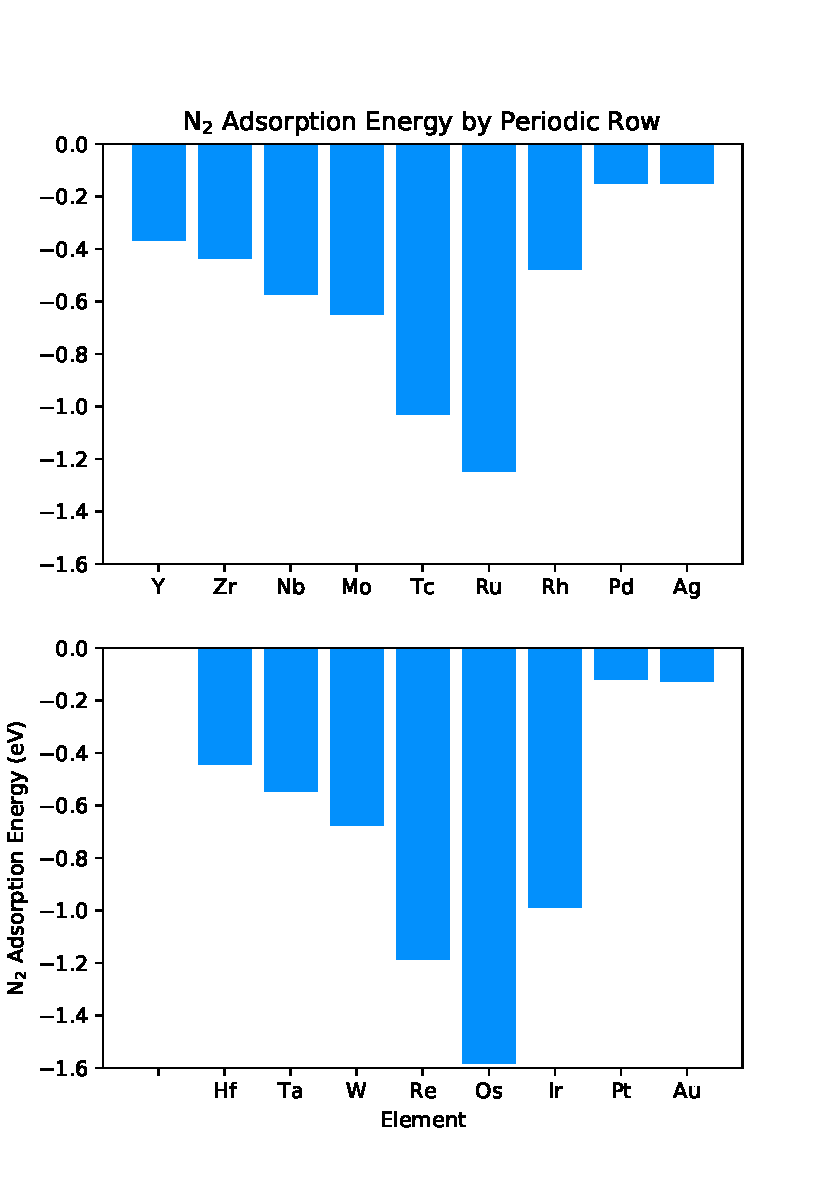
\includegraphics[width=0.5\textwidth]{Images/N2_adsorption_rows.pdf}
%    \caption{The adsorption of N$_2$ on 2+ metal substituent sites for d block elements in rows 4 and 5.}
%    \label{fig:N2_rows}
%\end{figure}

%\begin{figure}
%    \centering
%    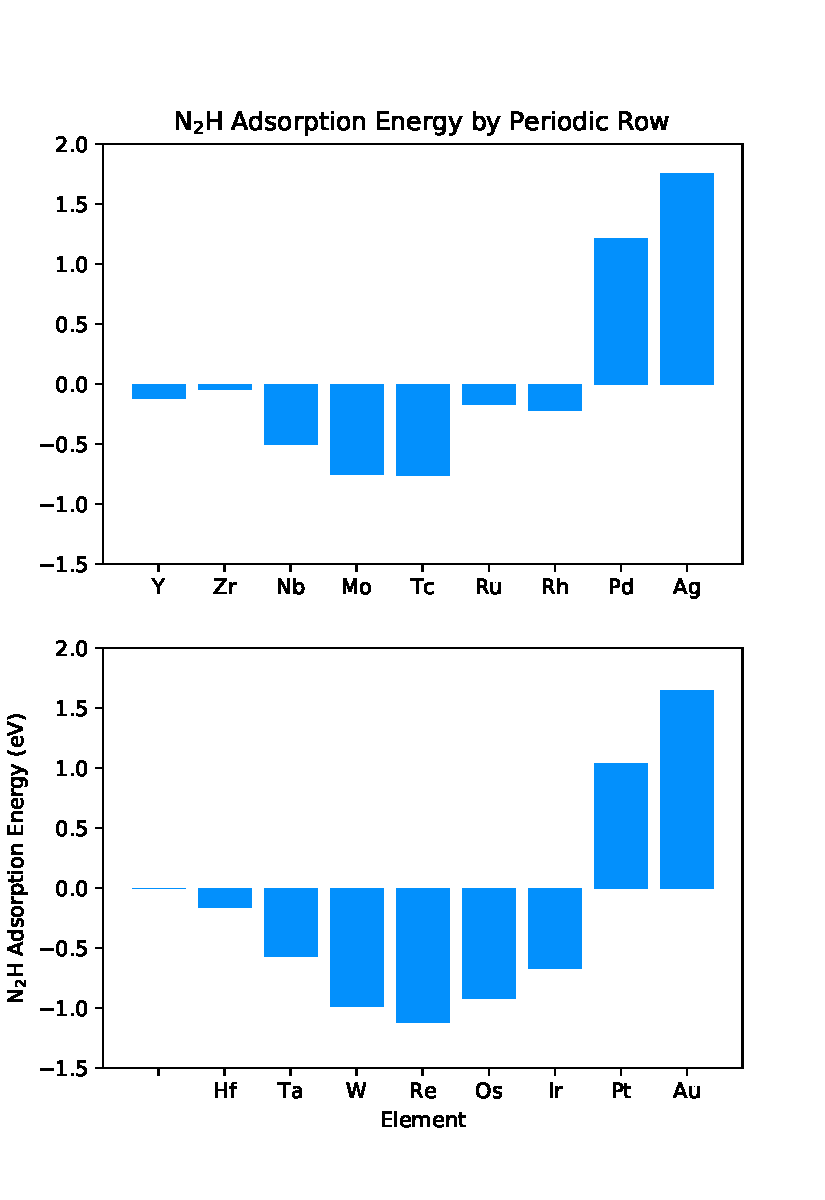
\includegraphics[width=0.5\textwidth]{Images/N2H_adsorption_rows.pdf}
%    \caption{The adsorption of N$_2$H on 2+ metal substituent sites for d block elements in rows 4 and 5}
%    \label{fig:N2H_rows}
%\end{figure}

\begin{figure}
    \centering
    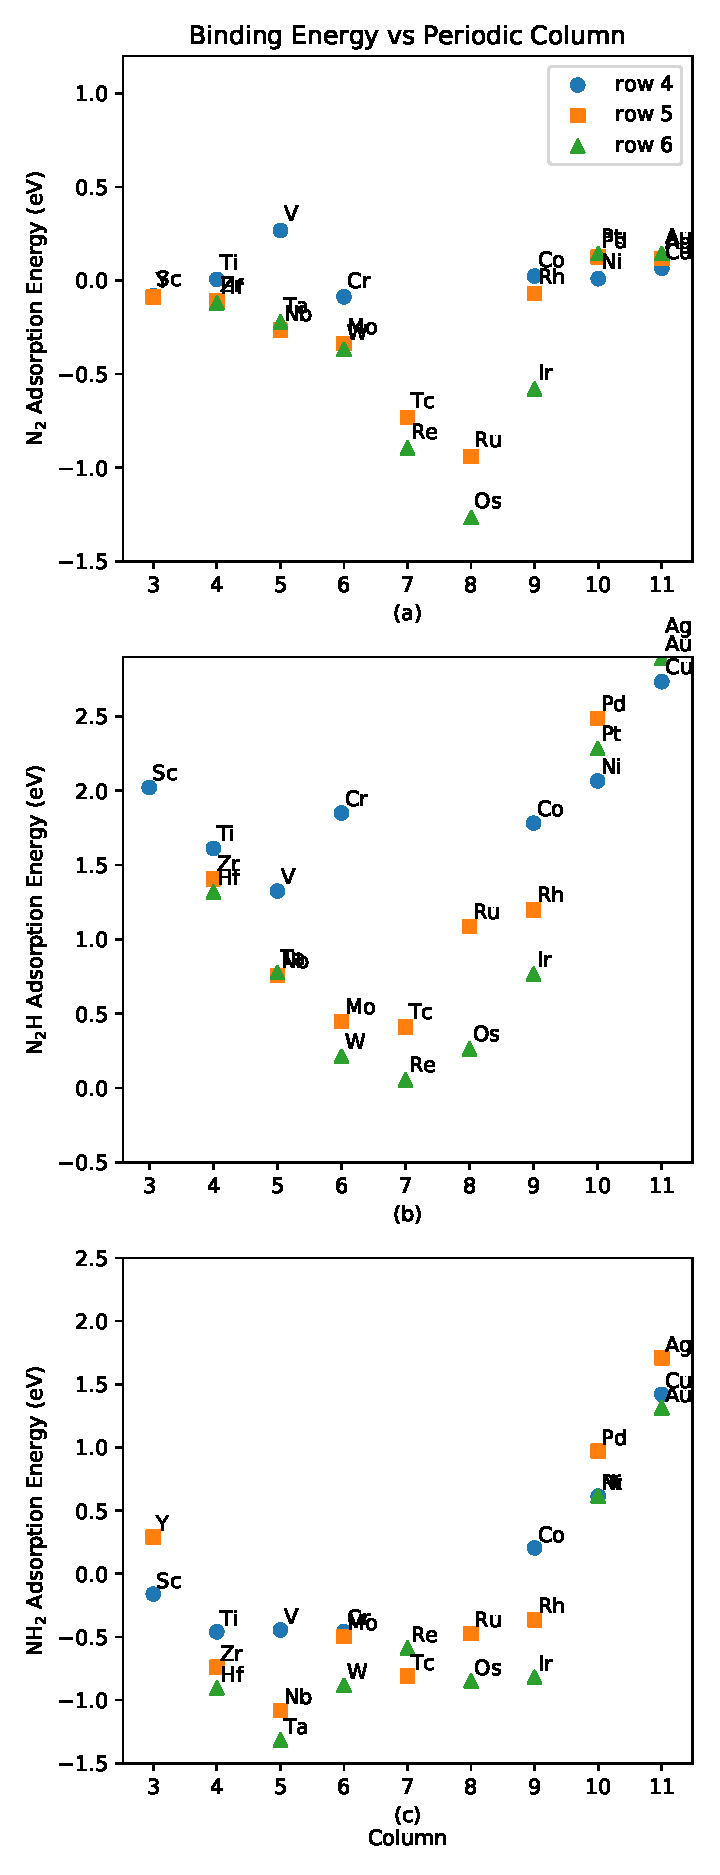
\includegraphics[width=0.4\textwidth]{Images/adsorption_rows.pdf}
    \caption{The binding energies of (a) N$_2$, (b) N$_2$H and (c) NH$_2$ plotted against the periodic column for 2+ metal substituent sites}
    \label{fig:column_trends}
\end{figure}

While the N$_2$, N$_2$H, and NH$_2$ binding observed deviates from the near-linear correlation expected from the \textit{d}-band model, we find a linear correlation between the binding energies and the \textit{d}-band contributions of the cohesive energies of the corresponding bulk systems (Figure \ref{fig:cohesive}). Cohesive Energy is defined as the change in energy associated with isolated, neutrally charged atoms being brought together to form a bulk material \cite{Laughlin_2014}. A metal's cohesive energy is made up of a \textit{d} contribution and a \textit{s} contribution (Eq. \ref{eq:cohesive}). Cohesive energies have generally been a measure of the ``bulk-nobleness'' of a metal \cite{Hammer_1995}, with higher cohesive energies correlating to a more noble character. The metals with the highest ``bulk-nobleness'' are in the center of the \textit{d}-block and resist corrosion due to the difficulty of breaking their strong metal-metal bonds. In our case, the inverse is true: the stronger the metal-metal bonds of the bulk material, the stronger the interaction between the metal and a given nitrogen species.

\begin{equation}
    E_{coh} = \epsilon_d + \epsilon_s
    \label{eq:cohesive}
\end{equation}
where $E_{coh}$ is the total cohesive energy, $\epsilon_d$ is the \textit{d} contribution and $\epsilon_s$ is the \textit{s} contribution.

%The \textit{d}-band cohesive energy of \textit{d}-block metals can be described by the Friedel Model \cite{1969TPom}. The key assumption of the Friedel model is that the \textit{d}-band is rectanglar in shape. In the Friedel model, electrons fill bonding \textit{d}-states in the first half of the \textit{d}-block, and anti-bonding \textit{d}-states in the second half, with the only difference between metals being the extent to which electrons fill the \textit{d}-band. The assumption of a square shape for the \textit{d}-band then yields a quadratic dependence in bond strength with respect to position on the periodic table \cite{1969TPom}.%, and is summarized in Equations \ref{eq:cohesive} and \ref{eq:d_band_cohesive}:

The correlation between \textit{d}-band contribution to cohesive energy and binding is the strongest for N$_2$H and NH$_2$ (Figure \ref{fig:cohesive}b-c). These two species show a relatively strong quadratic dependence (Figure \ref{fig:column_trends}b-c) suggesting that the bonding of nitrogen species to these substituent metals is similar to that of forming metal-metal bonds of the original bulk material. Thus, we hypothesize that the physics of nitrogen bonding to these substituent sites is similar to the bonding between single metal atoms and a bulk metal.
%but the trend also exists to some extent in NH$_2$ and N$_2$. 
A similar quadratic trend is seen for N$_2$ adsorption in Fig. \ref{fig:cohesive}a, though there are several outliers near the middle of the \textit{d}-block (Tc, Ru, Re, Os, Ir) that bind N$_2$ substantially stronger than predicted by the cohesive energy descriptor. The origin of this anomalously-high reactivity toward N$_2$ is not clear, though we note that the bonding mechanism changes between physisorption for early/late metals and chemisorption for more reactive metals, indicating that the quadratic trend may still hold for chemisorption.
%suggests that the simplistic Friedel model breaks down for N$_2$ binding on these reactive atoms, though the origins of this deviation are beyond the scope of this work.

The trends observed for site formation energy (Figure \ref{fig:d_band}) and nitrogen compound adsorption energy (Figure \ref{fig:cohesive}) differ qualitatively from trends observed in bulk metals. For single transition-metal dopant atoms, the \textit{d}-band center controls formation energy, while the cohesive energy controls adsorption energy. In bulk metals the inverse is true: the d-band center controls a material's ability to bind gas-phase species, whereas the cohesive energy controls how stable the material is \cite{Hammer_1995}. This trend has not been observed before for single-atom catalysts, but 
%However, this trend does not appear in the 4+ sites (see table SXX), implying the trend is not general.

%\begin{equation}
%    E_{coh} = \epsilon_d + \epsilon_s
%    \label{eq:cohesive}
%\end{equation}
%where $E_{coh}$ is the cohesive energy, $\epsilon_s$ is the \textit{s}-electron contribution to the cohesive energy (assumed to be constant for \textit{d}-block metals), and $\epsilon_d$ is the \textit{d}-electron contribution to the cohesive energy given by:

%\begin{equation}
%    \epsilon_d = \int^{E_F} (E_d-E)\rho(E)dE
%    \label{eq:d_band_cohesive}
%\end{equation}
%where $E_F$ is the Fermi level energy, $E_d$ is the energy associated with broadening the \textit{d}-band, and $\rho(E)$ is the \textit{d}-band density of states of the material. 

%The Friedel Model (Eq. \ref{eq:cohesive} and \ref{eq:d_band_cohesive}) and the \textit{d}-band model (Eq. \ref{eq:d_band}) both track the bonding and anti-bonding contributions of \textit{d} electrons. However, in the Friedel Model, the energy change is from fully isolated metal atoms to crystalline transition metals, and the \textit{d}-band is assumed to be a rectangular block. As a consequence, the bonding orbitals fill in the first half of the transition metal row, followed by the anti-bonding orbitals in the second half of the row. Thus, cohesive interactions strengthen in the first half of the row and weaken in the second half, creating a maxima when the \textit{d}-orbitals are half filled. The fact that N$_2$H binding follows a similar trend suggests that the $d$-band of the dopant metal atoms can be approximated by a rectangle, and that interactions with N$_2$H leads to a filling of bonding orbitals in the early transition metals, followed by filling of anti-bonding orbitals for the late transition metals. This is in contrast to the standard \textit{d}-band model, where only anti-bonding orbitals are created and filled due to the interaction between the \textit{d}-band and the molecular orbitals. 
%This suggests that the \textit{d}-band close to the fermi level is similarly rectangular.
%Additionally, the filling of the metal's \textit{d}-band for binding nitrogen species first fills up \textit{d}-bonding orbitals moving down the periodic row rather than merely anti-bonding orbitals as in the case for traditional \textit{d}-band model correlations. However, the lack of very tight correlation suggests that the assumptions the Friedel model makes about the \textit{d}-band do not hold for our system.
%when doped on a surface and the metal sublimating are similar.
%Thus, we hypothesize that these phenomena are governed by the same underlying physics. 


%There are also some significant deviations from the linear correlation for N$_2$H; however, the correlation between N$_2$H and N$_2$ adsorption is relatively strong (Fig. ???). 
%This finding indicates that there are correlations in the deviations from the simplistic model, although the N$_2$ adsorption on middle transition metals remains anomalously strong. The existence of linear scaling relations between nitrogen intermediates adsorbed at transition-metal dopants in TiO$_2$ is consistent with prior work on other adsorbates \cite{Xu_2015, Garc_a_Mota_2011, Yao_2017}. %, and we hypothesize that the latent correlation with the \textit{d}-band contributions to cohesive energies is a general descriptor for reactivity of single metal atoms in oxide surfaces.

%however the correlation is much less predictive due to several elements displaying much stronger binding than would be expected by this model. The low $R^2$ value of this correlation implies that the system is more complicated than the case of N$_2$H. Thus, for the case of N$_2$ binding, increasing cohesive energy predicting increased binding is only a general trend. 

%We need one final paragraph/figure for this section showing that the scaling relations (and hence the latent correlation with E_d,coh) holds for other nitrogen species.

%The existence of these trends shows the potential for tuning embedded metal sites to perform particular reactions. We based on our results and previous work \cite{Xu_2015,Garc_a_Mota_2011,Yao_2017} hypothesize that trends similar those found on TiO$_2$ apply to other metal oxides and crystal structures.

%In the  shows a reasonable correlation with the \textit{d}-band energy contribution to the cohesive energies of the bulk phases of the substituent metals as seen in Figure \ref{fig:N2H_cohesive}. This quantity may be obtained using equation \ref{eq:d_band_cohesive} below \cite{Gautier_1975}. The relationship implies that the \textit{d}-band contribution of the cohesive energy is related to the reactivity of the metal atom. Larger cohesive energy implies that the metal is more stabilized through bonding with itself, which can be thought of as the metal being more reactive. This trend does not match the one typically seen in the \textit{d}-band model, however the relationsh More reactive elements tend to lie in the center of the periodic row, due to their \textit{d}-band filling properties. The Friedel Model\cite{1969TPom} describes this in terms 


\begin{figure}
    \centering
    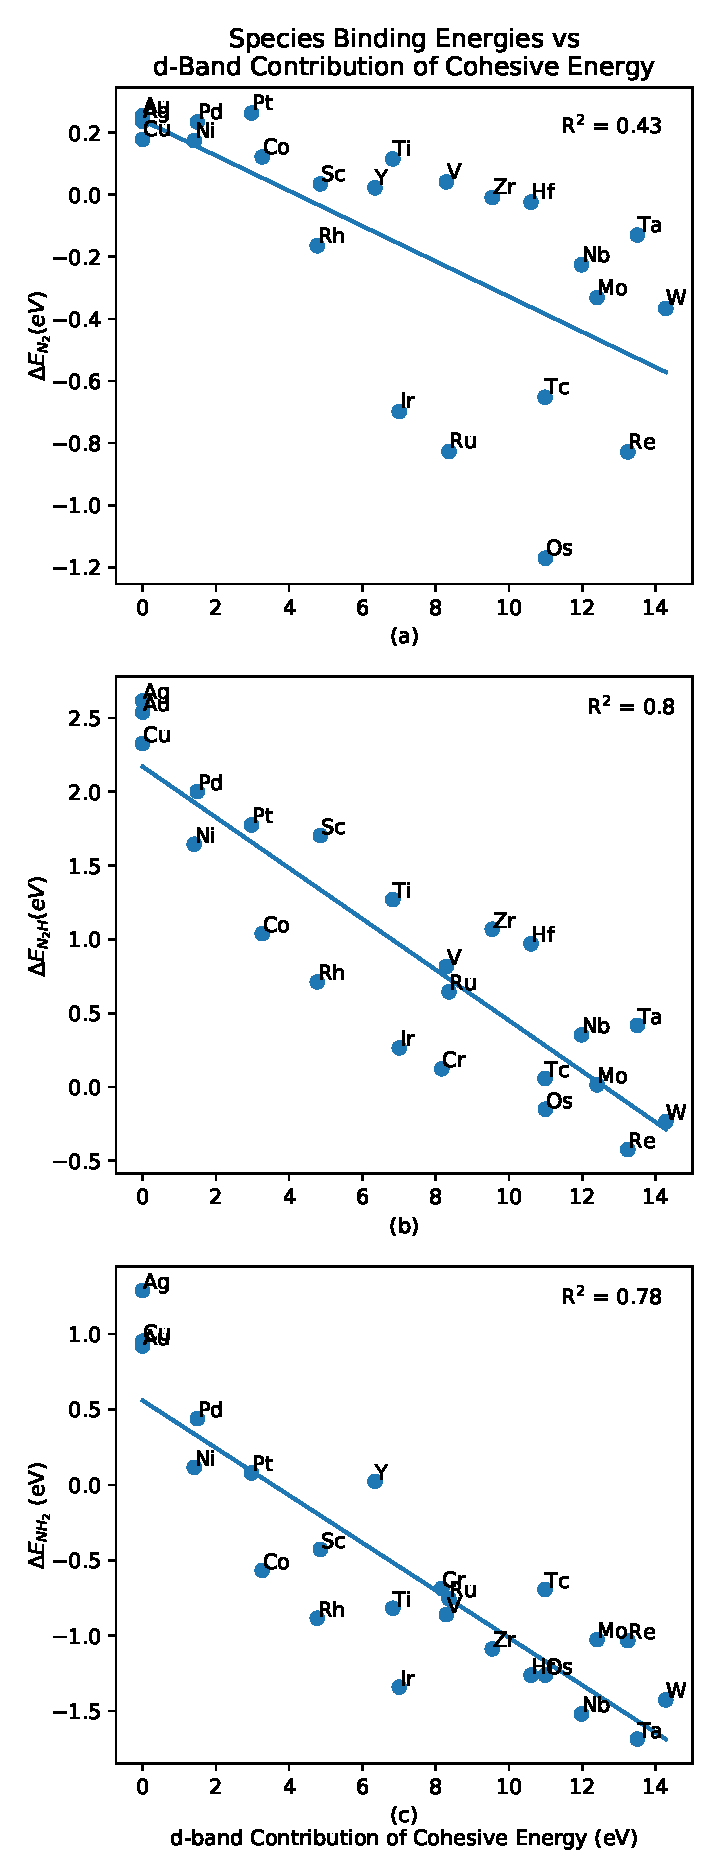
\includegraphics[width=0.4\textwidth]{Images/species_cohesive.pdf}
    \caption{the \textit{d}-band contribution to cohesive energies vs. the binding energies of (a) N$_2$, (b) N$_2$H, (c) NH$_2$ for 2+ metal substituent sites. The \textit{d}-band cohesive energy contributions obtained from Turchanin and Agraval \cite{Turchanin_2008}}
    \label{fig:cohesive}
\end{figure}

\subsection{Scaling Relationships in Binding and Reaction Energies}
\label{sec:scaling}

Hoskuldsson et al. \cite{Hoskuldsson_2017} previously found strong scaling relations between the binding of nitrogen compounds and the N$_2$H binding energy.  The binding energies of all species are fit using N$_2$H and N$_2$H as descriptors identified to assess the presence of scaling relations in our system. The results of this scaling analysis may be seen in Figure SXX. The scaling relations for this system are relatively moderate, with most having a root mean squared error of 0.2 eV. The N$_2$H and NH$_2$ were also used to fit scaling relationships for all electrochemical steps. The results of this analysis may be seen in Figure SXX. As with the scaling relationships for the binding of individual species, the scaling relationships chemical reactions are moderately predictive, havin a root mean square error of roughly 0.2 eV.

%The reason for these weak correlations is likely due to limitations in the computational methods selected. Specifically, the pseudopotentials selected \cite{SSSP_pseudos} may not be well suited to modeling this system, as they are highly heterogeneous in type, and are optimized to replicate bulk properties. The cells were also not allowed to relax, causing some systems to have strain effects, which can affect binding energies \cite{Xu_2015}. Additionally, GGA functionals are known to have difficulty modeling oxide materials \cite{}. However, the full cause of these inconsistencies is not known.

\subsection{Trends in Catalytic Activity for Nitrogen Reduction}
\label{sec:cat_trends}
The photocatalytic activity of doped TiO$_2$ surfaces can be assessed by computing the maximum thermodynamic barrier with electrons at the conduction band edge potential \cite{Comer_2018}, while the electrocatalytic activity of doped TiO$_2$ surfaces can be assessed by computing the thermodynamic limiting potential \cite{Norskov_2004,Garc_a_Mota_2011}. The computational hydrogen electrode (CHE) provides a route to computing the thermochemical potential of electrons at the TiO$_2$ surface (Sec. \ref{sec:PEC_methods}), and the resulting analysis provides only a thermodynamic picture of the reaction pathway. This analysis establishes a lower bound on the kinetics and correlates well with experimental trends in the literature\cite{Seh_2017}.

Computing the maximum barrier or limiting potential requires the free energies of each state along a given reaction pathway. However, the binding energy of N$_2$H has been previously identified to be the primary descriptor for a surface's ability to perform the nitrogen reduction reaction \cite{Hoskuldsson_2017, Montoya_2015}. Using the N$_2$H adsorption energies provides an initial estimate of the limiting potential that is a lower bound to the actual limiting potential, and hence provides a good starting point for screening. The N$_2$H adsorption energies were computed for all 2+ and 4+ defects, revealing prohibitive barriers of $>$1.5 eV for all 4+ sites (Table SXX) and a lack of clear trends as discussed in Sec. \ref{sec:reactivity}. For this reason, only 2+ sites were considered for limiting potential analysis. %However, some 2+ sites have reasonable N$_2$H binding energies, thus further thermodynamic pathway analysis was performed for 2+ sites.
The full thermodynamics of the N$_2$ reduction reaction pathways on all 2+ sites were calculated, allowing the generation of free energy diagrams for all possible reaction pathways (Fig. SXX-SYY, Table \ref{table:energies}). 
 



%To assess the nitrogen reduction reaction rates of these sites, two cases were considered: electrochemistry and photochemistry. 

%To simulate electrochemistry, the computational hydrogen electrode model (CHE) was employed. Thus, the effects of applied potential were taken into account with a factor of -eU, where e is the fundamental charge and U is the potential relative to CHE. To simulate the effect of excited electrons, the computational hydrogen electrode was used and the potential was set to that of the band edge of rutile TiO$_2$. %We therefore neglect the effects these metals could have on the photo-physical properties of the material. The free energy diagrams for each pathway considered are available in the supplementary information.

The electrochemical limiting potential was calculated for all surfaces to assess their ability to reduce N$_2$ under applied bias. The results are plotted against the NH$_2$ binding energy in Figure \ref{fig:NH2_limiting_pot}. This plot reveals a clear volcano relationship between the NH$_2$ binding energy and the limiting potential. In contrast to prior work by Hoskuldsson et. al.\cite{Hoskuldsson_2017} and Montoya et. al. \cite{Montoya_2015}, we find that the NH$_2$ binding energy is a slightly more reliable descriptor than N$_2$H binding; however these quantities are fundamentally linked by scaling relations (Section \ref{sec:scaling}), indicating that either descriptor can is valid. In this case, the limiting step shifts from NH$_2$ desorption on the left to N$_2$ hydrogenation on the right, with most dopants being limited by NH$_2$ desorption. This means that NH$_2$ adsorption energy directly controls the reactive side of the volcano, and explains why it is an accurate descriptor in this case. There are also a few dopants that deviate from the trend. 
%Notably, Ti (i.e. undoped TiO$_2$) is on the reactive side of the volcano, but the potential limiting step is N$_2$H formation\cite{Comer_2018, Hoskuldsson_2017}. Nonetheless, Ti fortuitously falls close to the trend predicted by the volcano plot. 
Notably, the potential limiting step of  Ru, Sc, Zr, Rh, and Ru are also limited by N$_2$H formation despite being on the reactive leg of the volcano.
%anomalously strong N$_2$ adsorption. On the other hand, Sc is simply an outlier on the NH$_2$ vs. N$_2$H scaling relation, causing its limiting potential to be under-estimated.

\begin{figure}
    \centering
    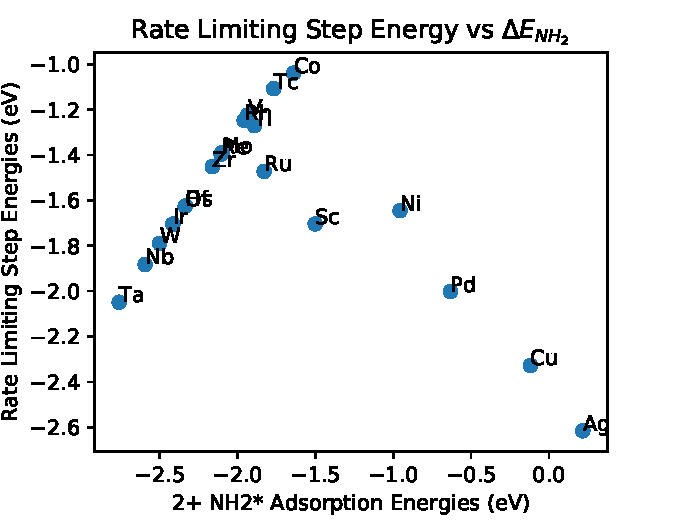
\includegraphics[width=0.4\textwidth]{Images/NH2_v_limiting_pot.pdf}
    
    \caption{The limiting potential vs the NH$_2$ Binding Energy. Any surface for which a full path was not available has been excluded.}
    \label{fig:NH2_limiting_pot}
\end{figure}

\begin{figure}
    \centering
    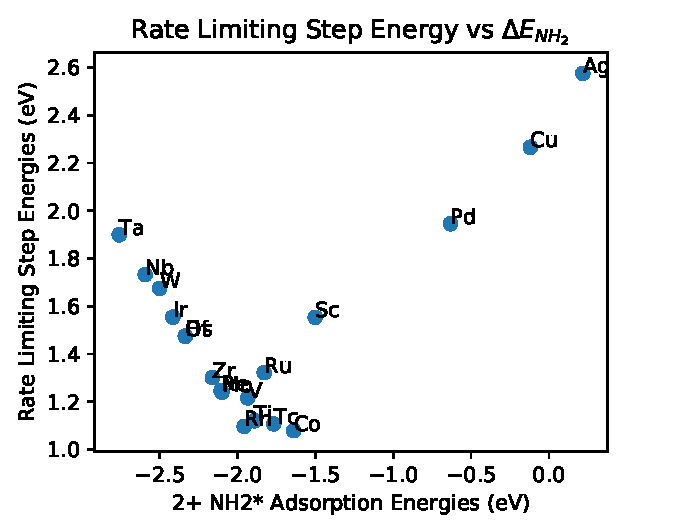
\includegraphics[width=0.4\textwidth]{Images/NH2_v_rate_limiting.pdf}
    
    \caption{The highest barrier observed vs the NH$_2$ Binding Energy. Any surface for which a full path was not available has been excluded.}
    \label{fig:NH2_limiting_bar}
\end{figure}

%The only element not following this trend is Ti, whose limiting step is also N$_2$ hydrogenation. This may not be surprising, as electronic interactions between the doping metal and the host metal atoms are known to have an impact on the chemistry of dopant sites, and this particular interaction is absent in the case of Ti \cite{Xu_2015}.\todo{does that make any sense?}. Additionally, Ru and Sc appear to be abnormally unreactive with respect to the trend in the volcano plot.

Overall, the results suggest that several dopants are capable of improving the performance over pure TiO$_2$. The elements that show significant improvement are Tc, Co, Mo, V, Rh, and Re. Tc sits at the top of the volcano. The high activity of Tc presents a serious problem for experimental testing or practical application since Tc is a scarce, synthetically produced, radioactive element. In addition, the active sites may be challenging to synthesize due to their relatively high formation energy (Fig. \ref{fig:d_band}). 

On the other hand, the relatively low limiting potential of Co, Mo, V, Rh, and Re are promising results. Co, Mo, and V are relatively inexpensive and abundant, whereas Re and Rh are relatively more expensive. These materials may present good opportunities for improving catalytic rates on TiO$_2$. However, the formation energy of the surface site may still present an issue since these active sites are relatively unstable compared to their respective bulk metals (Fig. \ref{fig:d_band}), but synthesis strategies that create meta-stable sites may be feasible. Moreover, the adsorption of N$_2$ at the Co site is endergonic, which lead to difficulties achieving substantial N$_2$* concentrations under competitive adsorption with H$_2$O. %Nonetheless, the results indicate that Co is the most promising dopant for improving electrocatalytic performance of TiO$_2$.
%Discouragingly, one of the species also near the top of the volcano is the host metal of the oxide material, Ti. This means that substituting other metals will only yield moderate improvements on rates of reaction for electrocatalysis. However, Co lowers limiting potential by 0.2V and is inexpensive and abundant making it a good candidate for experimental investigation.

A second consideration when assessing a surface's ability to catalyze a reaction electrochemically is the largest thermochemical barrier. Since some steps do not involve electron transfers (known as thermochemical steps) at the limiting potential the rate begins to be dominated by these thermochemical steps. The largest thermochemical barriers for each surface can be seen in figure SXX. This analysis reveals that NH$_3$ is bound very tightly on most surfaces, causing the desorption of NH$_3$ into the gas phase to become rate-limiting. However, the current analysis is done entirely in the gas phase. The effects of solvation that exist in liquid phase electrochemical cells may lower the energy required to desorb NH$_3$. The high thermochemical barriers NH$_3$ desorption introduces may indicate that surfaces with higher limiting potentials that are controlled by N$_2$ hydrogenation are preferable, due to the connection between these quantities through scaling relations (see Section \ref{sec:scaling}). This consideration can prevent selecting surface sites that will be poisoned by NH$_3$.

We assess the ability of dopant metals to improve photocatalytic nitrogen reduction by computing the largest thermodynamic barrier at a reductive potential equal to the conduction band edge of TiO$_2$ (approximately -0.15 V vs. RHE \cite{Nozik_1996}). For this analysis, we consider both electrochemical and thermochemical barriers. This approach assumes that the conduction band edge of TiO$_2$ is not significantly affected by the presence of the dopant, and neglects improvements in other bulk photochemical properties such as charge separation or carrier lifetime. Nonetheless, it provides a good starting point for assessing the impact of dopant metals on the surface catalytic properties.
The highest thermodynamic barrier for the best reaction pathway is plotted vs. the NH$_2$* binding energy in Figure \ref{fig:NH2_limiting_bar}. This quantity is different from the electrochemical limiting potential, as it includes non-electrochemical steps in addition to electrochemical steps. The thermodynamics of the electrochemical steps are improved by the reductive potential of excited electrons, while the chemical surface steps are unaffected. The energy of NH$_3$* and  NH$_2$* are roughly equal for most studied metals, so the slight change in the potential has a limited effect on metals on the left side of the plot. This lack of improvement is because the desorption of NH$_3$ (a non-electrochemical step) rapidly becomes rate-limiting. Surfaces where N$_2$ hydrogenation is rate-limiting shift to be slightly more favorable, effectively shifting the right side of the volcano downward. This shift leads to minimum thermodynamic barriers of 0.93 eV, 0.90 eV, 0.89 eV, 0.73 eV, for Zr, Co, Mo, and  Rh, respectively. The reasonable thermodynamics of these surfaces suggests that if kinetic barriers are very low, then photocatalytic nitrogen reduction may by promoted by 2+ dopant sites of these metals, though rates are still expected to be low relatively.

To better understand how the binding energies of the two primary species affect the limiting potential, the fits of the scaling relations (see Figure SXX) were used to generate a two dimensional volcano plot. The results can be seen in Figure \ref{fig:2d_plot}. As with the scaling relations, the root mean squared error of the predicted limiting potential in Figure \ref{fig:2d_plot} is roughly 0.2V.


\begin{figure}
    \centering
    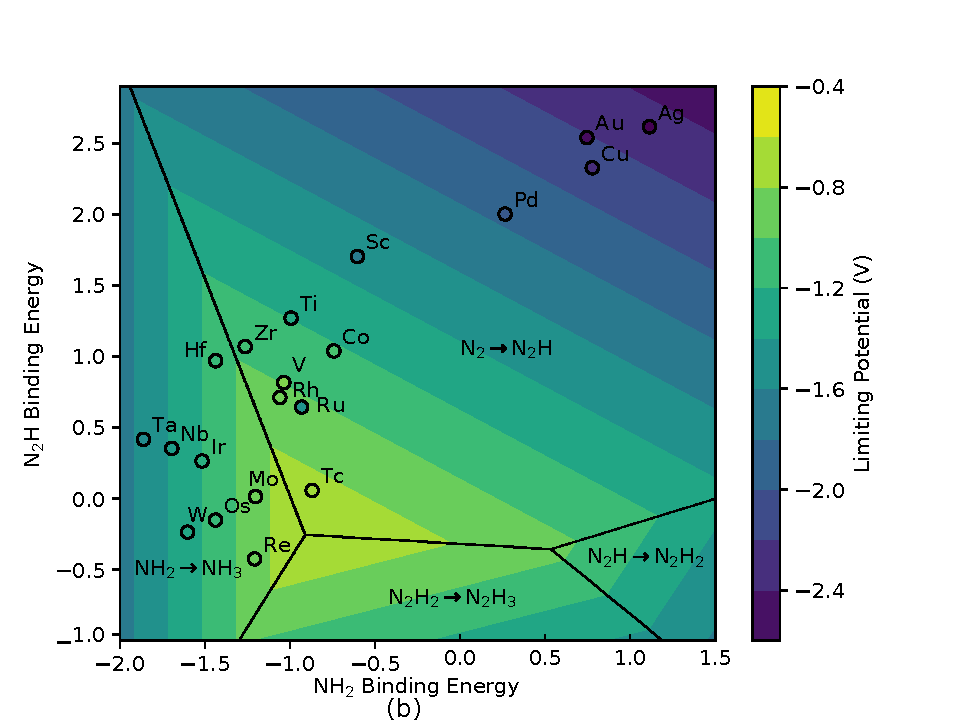
\includegraphics[width=0.55\textwidth]{Images/2d_scaling_plot.pdf}
    \caption{A two dimensional volcano plot using N$_2$H and NH$_2$ as descriptors for the studied systems.}
    \label{fig:2d_plot}
\end{figure}

Experimental observations can provide further insight into the computational predictions. Several prior reports have investigated transition-metal dopants for enhancing photocatalytic ammonia production on TiO$_2$ \cite{Schrauzer_1977, Ranjit_1996, Hirakawa_2017}. Interestingly Schrauzer et al. reports increases in ammonia yield in the presence of Co and Mo dopants \cite{Schrauzer_1977}, though this report comes from the early literature and rigorous controls \cite{Greenlee_2018} or isotopic labeling studies \cite{Andersen_2019} were not included. Moreover, the same report revealed enhanced rates for Fe and Ni, so the confirmation of the prediction regarding the former two should be treated with caution. The rate enhancement for noble metals such as Ru, Rh, Pt, and Pd is conflicting even in the early literature, with Schrauzer and Guth reporting no enhancement \cite{Schrauzer_1977}. However, Ranjit et al. reported enhancement for all noble metals with the most significant improvement for Ru \cite{Ranjit_1996}. In all of these systems, the metal dopants were incorporated via co-precipitation, and catalysts were polycrystalline TiO$_2$, indicating that the metals may also enhance yields via charge separation, mediation of crystallization, or other mechanisms\cite{Medford_2017}. Hirakawa et al. added Ru, Pt, and Pd to pre-synthesized TiO$_2$ particles and reported no significant improvement in the reaction rates \cite{Hirakawa_2017}. These experiments are more consistent with the computational model system used in this study since only surface properties are affected, and the results are consistent with the prediction that these noble metals will not affect the rate. However, further systematic and well-controlled experiments that characterize the state of the metal incorporation in the TiO$_2$ surface are required to validate the predicted trends.

%The lack of improvement in the rate of reaction with the addition of Ru, Pt, and Pd in the case of photocatalysis also agrees with the previous experimental findings by Hirakawa et. al.\cite{Hirakawa_2017}. They report no improvements in reaction rates when metals are bound to the TiO$_2$ surface.




%These results highlight the challenge of improving reaction rates for nitrogen fixation, indicating that more creative strategies must be employed. While have not considered the possible effects of metals on TiO$_2$'s bulk photochemical properties such as charge separation and carrier lifetime we believe this provides a starting point for engineering surface segregated metal dopants. In future, we could imagine engineering oxide structures with metal dopants in the bulk structure that improve photochemical properties and surface segregated metal dopants that improve reaction kinetics.



\section{Conclusions}
The stability of metal dopant surface sites and their effects on the reaction thermodynamics of N$_2$ reduction on rutile (110) are studied using DFT. We find that the formation energy of these doped surface states is strongly related to the location of the \textit{d}-band center of the substituted metal, with a trend consistent with the \textit{d}-band model. We also find a correlation between the cohesive energy of metals and their N$_2$H and NH$_2$ binding energy on the surface, suggesting that the bonding of nitrogen species is similar to that of bulk metals. Finally, we investigate the effects of dopant sites on the full reaction pathways for 2+ sites on all studied metals. We find a clear volcano relationship between NH$_2$ binding and both the electrochemical limiting potential and the highest thermodynamic barrier for photocatalytic reactions. The formation of Co and Mo 2+ sites is proposed to yield a slight improvement of reaction rates in both electrocatalysis and photocatalysis. Other metals commonly used in catalysis such as Pt, Ir, and Pd, are predicted to have a limited or detrimental effect on the surface catalytic properties of TiO$_2$ for nitrogen reduction. This suggests that the role of metal dopants in photocatalytic ammonia synthesis by TiO$_2$ is likely related to modifications of bulk properties in most cases. However, the existence of clear trends in the formation energy and reactivity of single metal atom dopants toward nitrogen intermediates suggests that computational design of metal-doped oxide materials is a promising strategy for other oxide systems and/or other nitrogen conversion reactions.


%We also show that metal dopant sites possess a substantial ability to modify reaction thermodynamics on the surface. For this reason, generating metal dopant sites on the surface is a potential path forward for improving reaction rates on metal oxide surfaces.


\section{Methods}
\label{sec:methods}

\subsection{Density Functional Theory Calculations}
All first principles calculations are performed in the Quantum Espresso software package \cite{QE-2009}.
The TiO$_2$ slabs and atomistic images are created using the Atomic Simulation Environment (ASE) package \cite{Hjorth_Larsen_2017}.  Spin polarization is used in all simulations to ensure the lowest energy spin state is obtained for each site. The BEEF-vdW functional \cite{Wellendorff_2012} is used with plane wave cutoff of 400 eV and a Monkhorst-Pack k-point grid spacing of 4$\times$4$\times$1 \cite{Monkhorst_1976}. The effciency versions of the standard solid state psuedopotentials \cite{SSSP_pseudos} (SSSP) are used for all calculations because of their high reported accuracy \cite{Lejaeghereaad3000}. The convergence threshold is set at $10^{-6}$ eV and Fermi-Dirac smearing of 0.1 eV is used. All structures are converged to a maximum force smaller than 0.05 eV/A using the BFGS line search algorithm. Adsorption energies are obtained from the DFT calculations by subtracting the energy of a clean slab and the energy of the free gas molecule from the energy of the gas adsorbed to the slab:
\begin{equation}
E_{adsorption} = E_{slab+adsorbate} - E_{slab} - E_{adsorbate}
\end{equation}
%The error of DFT calculations tends to be in the order of magnitude of 0.5 eV \cite{Gautier_2015}. 

\subsection{Thermochemistry}
%\cite{ase-paper,Reuter_2005}

To calculate the adsorption energy at standard temperature and pressure, the thermochemistry package from ASE is used \cite{ase-paper}. Free gasses are approximated in the ideal gas limit, and adsorbed gasses in the harmonic limit \cite{Reuter_2005}. A frequency cutoff of 33 cm$^{-1}$ for low frequency modes was selected. The vibrational mode for all metals were assumed to be approximately the same as those of the respective species adsorbed to the oxygen vacant TiO$_2$ (110) surface, thus the same thermodynamic correction values are applied to all species of the same type.

\subsection{Photochemistry}
\label{sec:PEC_methods}
The photochemistry has been treated using the methods outlined by Hellman et. al. \cite{Hellman2017}. Within this framework, the effects of excited states are neglected allowing the treatment of excited electrons and holes using the computational hydrogen electrode model (CHE). In this formalism, the reference electrode is set by setting the free energy of hydrogen evolution reaction (HER) to zero:
\begin{equation}
    H^+ + e^- \rightarrow H_2;\; \Delta G = 0\:at\: U = 0
\end{equation}

The potentials of electrons and holes are set at the value of the band edges of the rutile \cite{Nozik_1996}.

\subsection{Model Surface Generation}
 The surfaces are constructed with 4 TiO$_2$ tri-layers (bottom 2 layers constrained to bulk positions), with a 1$\times$2 supercell repeat. The pristine slab totals 48 atoms, with 4 Ti and 8 O per tri-layer. 6 \A{} of vacuum are added on both top and bottom of the slab and a dipole corrections is applied in the $z$ direction\cite{Dipole_paper}. The lattice parameters of the unit cells are fixed at the calculated value for pure rutile TiO$_2$. 2+ sites were created by replacing the six-fold titanium site with the substituent metal and removing a single bridging oxygen (see Figure \ref{fig:ex_slab}.) 4+ sites were generated by replacing the five-fold titanium site with the substituent metal. The adsorption site was selected to directly over the substituent metals. 

\section{Acknowledgements}
We would like to thank Fuhzu Liu and Gabriel Gusm\~ao for their comments and suggestions for improving this manuscript.

\bibliographystyle{abbrv}
\bibliography{main}
\appendix
Supplementary Information
\onecolumn
\begin{table}
\begin{center}
\begin{tabular}{| c | c | c | c | c | c | c | c | c | c | c | c | c | c |}
\hline
Element & H$_2$NNH$_2$ & HNNH & N & N$_2$ & N$_2$H & N$_2$H$_2$ & N$_2$H$_3$ & NH & NH$_2$ & NH$_3$ & Formation Energy\\
\hline

Rh & 1.16 & 1.3 & 1.86 & -0.16 & 0.71 & 0.85 & 0.44 & 1.34 & -0.88 & -0.87 & 6.01 \\
Ir & 0.82 & 0.74 & 1.03 & -0.7 & 0.26 & 0.19 & -0.01 & 0.54 & -1.34 & -1.2 & 7.07 \\
Ru & 0.82 & 0.76 & 0.48 & -0.83 & 0.64 & 0.17 & 0.57 & 0.86 & -0.76 & -1.13 & 5.45 \\
W & 1.25 & 0.84 & -1.8 & -0.37 & -0.24 & -0.73 & 0.01 & -1.06 & -1.43 & -0.8 & 3.99 \\
Tc & 1.03 & 0.95 & -0.87 & -0.65 & 0.06 & 0.27 & 0.65 & 0.52 & -0.69 & -0.92 & 4.58 \\
Zr & 1.23 & 1.39 & 1.71 & -0.01 & 1.07 & 0.74 & 0.35 & 0.16 & -1.09 & -0.88 & -0.51 \\
Re & 0.95 & 0.67 & -1.5 & -0.83 & -0.42 & -0.15 & 0.32 & -0.18 & -1.03 & -0.96 & 5.06 \\
Pd & 1.53 & 2.12 & 3.55 & 0.23 & 2.0 & 2.25 & 1.67 & 2.5 & 0.44 & -0.22 & 6.08 \\
Ti & 1.42 & 1.64 & 1.73 & 0.11 & 1.27 & 0.85 & 0.61 & 0.37 & -0.82 & -0.6 & 0.0 \\
Cu & 1.33 & 2.07 & 4.51 & 0.18 & 2.33 & 2.4 & 1.65 & 3.41 & 0.95 & -0.45 & 6.55 \\
Ni & 1.75 & 1.94 & 3.35 & 0.17 & 1.64 & 1.9 & 1.09 &  & 0.12 & -0.43 & 5.58 \\
Os & 0.61 & 0.39 & -0.7 & -1.17 & -0.15 & -0.36 & 0.06 & 0.06 & -1.26 & -1.29 & 6.31 \\
Ta & 1.1 & 0.31 & -0.99 & -0.13 & 0.42 & -0.32 & -0.22 & -0.95 & -1.69 & -0.85 & 1.69 \\
Hf & 1.21 & 1.32 & 1.59 & -0.02 & 0.97 & 0.6 & 0.2 & 0.02 & -1.26 & -0.95 & -0.92 \\
Sc & 1.06 & 1.76 & 3.51 & 0.03 & 1.7 & 1.59 & 1.0 & 2.18 & -0.43 & -0.76 & -1.71 \\
Co & 1.14 & 1.53 & 2.34 & 0.12 & 1.04 & 1.05 & 0.78 & 1.82 & -0.57 & -0.72 & 4.49 \\
V & 1.43 & 1.5 & -0.33 & 0.04 & 0.82 & 0.38 & 0.55 & 0.17 & -0.86 & -1.03 & 2.48 \\
Y & 1.01 & 1.69 & 2.72 & 0.02 &  & 2.0 & 1.34 & 2.58 & 0.02 & -0.77 & -1.38 \\
Au & 1.68 & 2.36 & 4.05 & 0.25 & 2.54 & 2.82 & 2.15 & 2.95 & 0.92 & -0.08 & 8.18 \\
Mo & 1.27 & 1.11 & -1.2 & -0.33 & 0.01 & -0.08 & 0.39 & -0.24 & -1.03 & -0.75 & 3.26 \\
Ag & 1.44 & 2.33 & 5.3 & 0.24 & 2.62 & 2.65 & 2.04 & 3.83 & 1.29 & -0.18 & 7.28 \\
Pt &  & 2.16 & 2.77 & 0.26 & 1.78 & 2.06 & 1.44 & 1.69 & 0.08 & -0.09 & 6.86 \\
Nb & 1.23 & 0.43 & -1.04 & -0.23 & 0.35 & -0.36 & -0.04 & -0.84 & -1.52 & -0.86 & 1.5 \\
\hline
\end{tabular}
\end{center}
\caption{The calculated relative energies of all 2+ surface species on all metal substituents at standard state. All energies are referenced with respect to N$_2$ gas and H$_2$ gas at 300K and 1 bar of pressure. Blank spaces represent calculations that could not be converged}
\label{table:energies}
\end{table}

\begin{table}
\begin{center}
\begin{tabular}{| c | c | c | c |}
\hline
Element & N$_2$ & N$_2$H & Formation Energy \\
\hline
Rh & -0.14 & 2.22 & 8.71 \\
Ir & -0.39 & 2.1 & 9.12 \\
Ru & -0.0 &  & 7.5 \\
W & 0.13 & 2.37 & 4.36 \\
Tc & 0.12 &  & 5.88 \\
Zr & 0.07 & 2.46 & -0.75 \\
Re & 0.12 &  & 5.9 \\
Pd & -0.01 & 1.7 & 9.88 \\
Fe & -0.12 &  & 8.4 \\
Ti & 0.16 & 2.54 & -0.0 \\
Cu & 0.22 &  & 10.16 \\
Ni & 0.2 & 1.75 & 9.29 \\
Os & -0.22 & 1.96 & 7.69 \\
Ta & 0.1 & 2.37 & 1.39 \\
Hf & 0.06 & 2.43 & -1.22 \\
Sc & 0.08 & 2.34 & 0.63 \\
Co & 0.2 &  & 7.42 \\
V & 0.19 & 2.81 & 2.82 \\
Y & 0.04 & 2.6 & 1.1 \\
Au & 0.27 & 2.23 & 11.22 \\
Mo & 0.14 &  & 3.95 \\
Ag & 0.24 &  & 11.09 \\
Pt & -0.34 & 1.77 & 10.08 \\
Nb & 0.11 & 2.45 & 1.4 \\
\hline
\end{tabular}
\end{center}
\caption{The calculated relative energies of all 4+ surface species on all metal substituents at standard state. All energies are referenced with respect to N$_2$ gas and H$_2$ gas at 300K and 1 bar of pressure. Blank spaces represent calculations that could not be converged}
\hline
\end{table}

\begin{table}
\begin{center}
\begin{tabular}{| c | c |c |}
\hline
Element & Limiting Potential & Limiting Step \\
\hline
Sc & -1.7 & N$_2$ $\rightarrow$ N$_2$H*\\
Ti & -1.27 & N$_2$ $\rightarrow$ N$_2$H*\\
V & -0.82 & N$_2$ $\rightarrow$ N$_2$H*\\
Co & -1.04 & N$_2$ $\rightarrow$ N$_2$H*\\
Ni & -1.64 & N$_2$ $\rightarrow$ N$_2$H*\\
Cu & -2.33 & N$_2$ $\rightarrow$ N$_2$H*\\
Zr & -1.08 & N$_2$* $\rightarrow$ N$_2$H*\\
Nb & -1.38 & NH$_2$*+NH$_3$ $\rightarrow$ 2NH$_3$\\
Mo & -0.89 & NH$_2$*+NH$_3$ $\rightarrow$ 2NH$_3$\\
Tc & -0.71 & N$_2$* $\rightarrow$ N$_2$H*\\
Ru & -1.47 & N$_2$* $\rightarrow$ N$_2$H*\\
Rh & -0.88 & N$_2$* $\rightarrow$ N$_2$H*\\
Pd & -2.0 & N$_2$ $\rightarrow$ N$_2$H*\\
Ag & -2.62 & N$_2$ $\rightarrow$ N$_2$H*\\
Hf & -1.12 & NH$_2$*+NH$_3$ $\rightarrow$ 2NH$_3$\\
Ta & -1.55 & NH$_2$*+NH$_3$ $\rightarrow$ 2NH$_3$\\
W & -1.29 & NH$_2$*+NH$_3$ $\rightarrow$ 2NH$_3$\\
Re & -0.9 & NH$_2$*+NH$_3$ $\rightarrow$ 2NH$_3$\\
Os & -1.12 & NH$_2$*+NH$_3$ $\rightarrow$ 2NH$_3$\\
Ir & -1.2 & NH$_2$*+NH$_3$ $\rightarrow$ 2NH$_3$\\
Au & -2.48 & N$_2$ $\rightarrow$ N$_2$H*\\
\hline
\end{tabular}
\end{center}
\caption{The limiting potentials and limiting steps for each dopant metal on 2+ surfaces}\label{table:limiting_steps}\end{table}\hline
\end{table}

\begin{table}
\begin{center}
\begin{tabular}{| c | c |c |}
\hline
Element & Limiting Potential & Limiting Step \\
\hline
Sc & 0.44 & NH$_3$*+NH$_3$ $\rightarrow$ 2NH$_3$\\
Ti & 0.68 & NH$_3$*+NH$_3$ $\rightarrow$ 2NH$_3$\\
V & 0.72 & NH$_3$*+NH$_3$ $\rightarrow$ 2NH$_3$\\
Co & 0.43 & NH$_3$*+NH$_3$ $\rightarrow$ 2NH$_3$\\
Ni & 0.17 & N$_2$ $\rightarrow$ N$_2$*\\
Cu & 1.25 & H$_2$NNH$_2$* $\rightarrow$ 2NH$_2$*\\
Zr & 0.95 & NH$_3$*+NH$_3$ $\rightarrow$ 2NH$_3$\\
Nb & 1.38 & NH$_3$*+NH$_3$ $\rightarrow$ 2NH$_3$\\
Mo & 0.89 & NH$_3$*+NH$_3$ $\rightarrow$ 2NH$_3$\\
Tc & 0.61 & NH$_3$*+NH$_3$ $\rightarrow$ 2NH$_3$\\
Ru & 0.82 & NH$_3$*+NH$_3$ $\rightarrow$ 2NH$_3$\\
Rh & 0.75 & NH$_3$*+NH$_3$ $\rightarrow$ 2NH$_3$\\
Pd & 0.54 & H$_2$NNH$_2$* $\rightarrow$ 2NH$_2$*\\
Ag & 1.48 & H$_2$NNH$_2$* $\rightarrow$ 2NH$_2$*\\
Hf & 1.12 & NH$_3$*+NH$_3$ $\rightarrow$ 2NH$_3$\\
Ta & 1.55 & NH$_3$*+NH$_3$ $\rightarrow$ 2NH$_3$\\
W & 1.29 & NH$_3$*+NH$_3$ $\rightarrow$ 2NH$_3$\\
Re & 0.9 & NH$_3$*+NH$_3$ $\rightarrow$ 2NH$_3$\\
Os & 1.12 & NH$_3$*+NH$_3$ $\rightarrow$ 2NH$_3$\\
Ir & 1.2 & NH$_3$*+NH$_3$ $\rightarrow$ 2NH$_3$\\
Au & 0.82 & H$_2$NNH$_2$* $\rightarrow$ 2NH$_2$*\\
\hline
\end{tabular}
\end{center}
\caption{The largest thermodynamic barrier and correspinding steps for each dopant metal on 2+ surfaces}\label{table:limiting_steps}\end{table}\begin{figure}
\centering
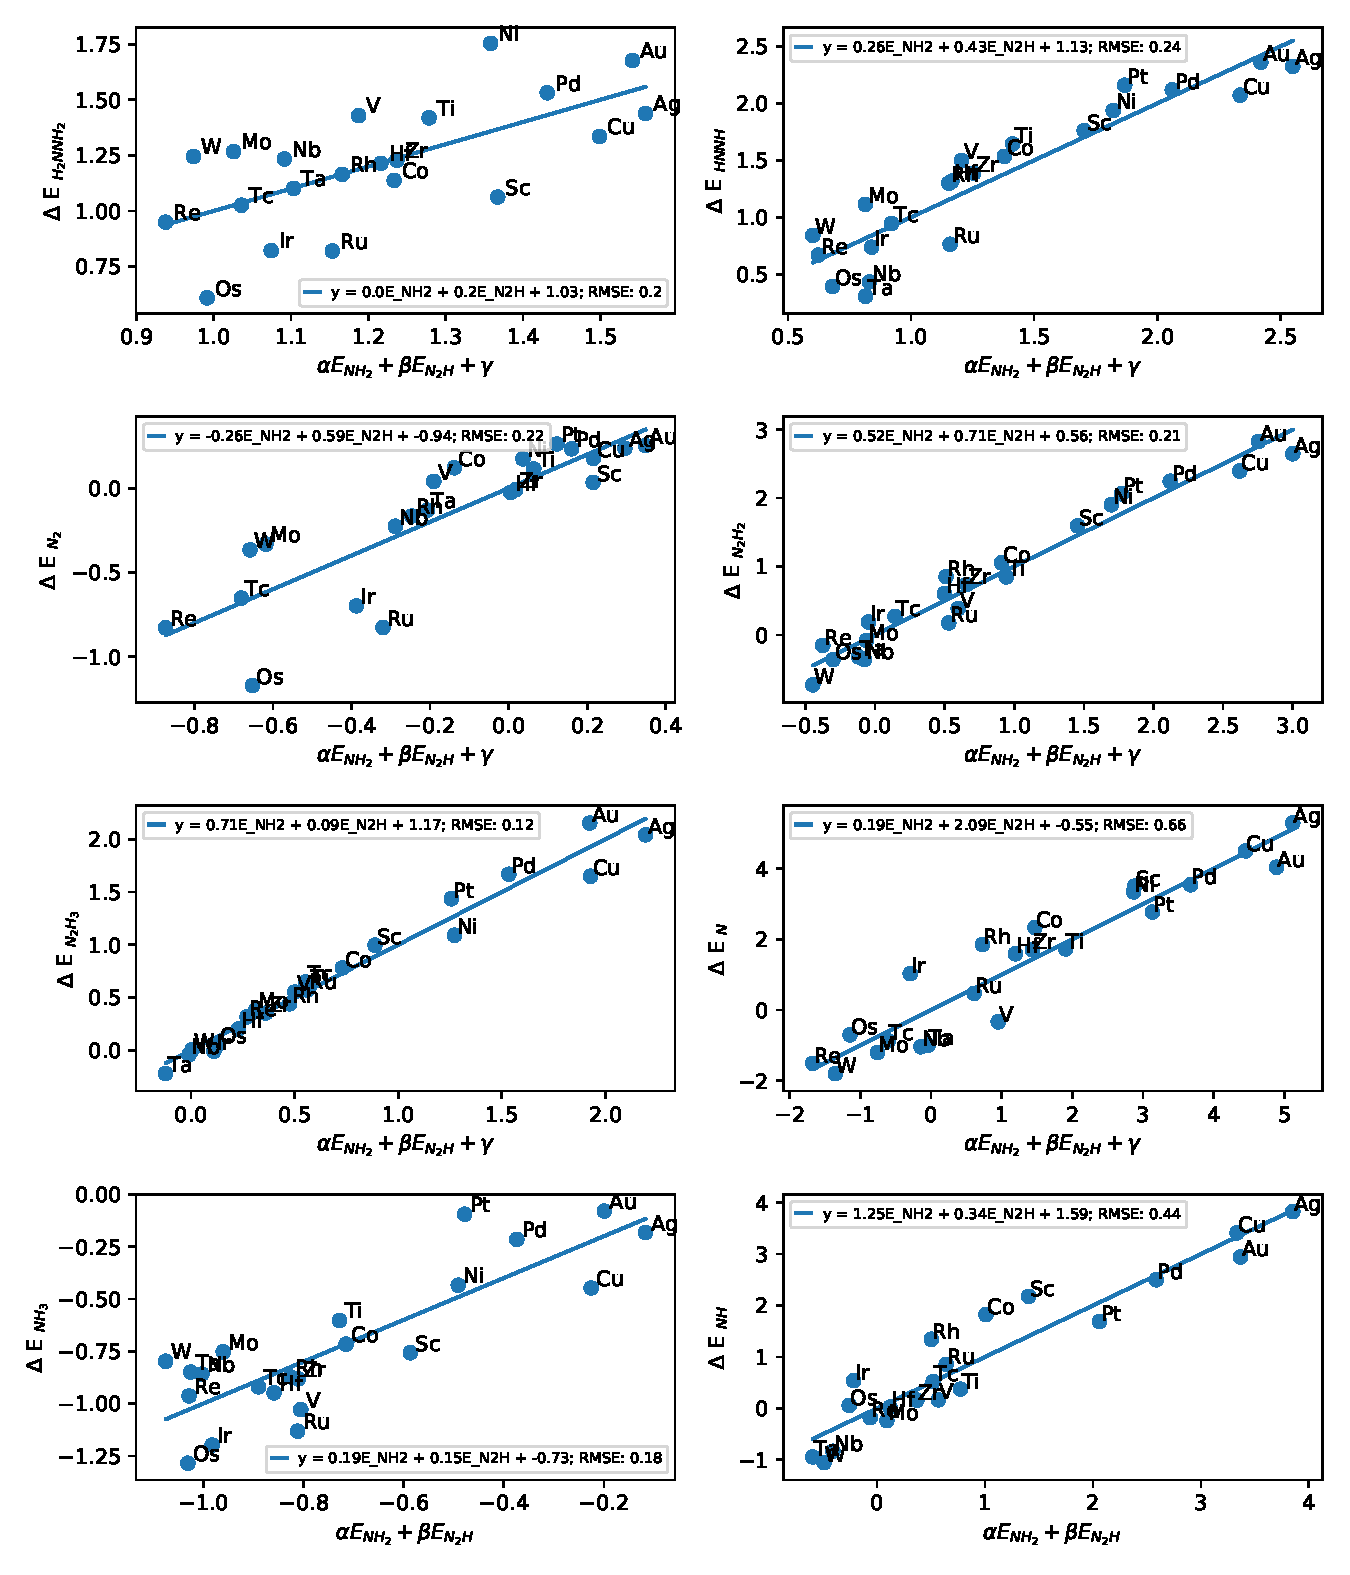
\includegraphics[width=0.8\linewidth]{Images/scaling_species.pdf}
\caption{The calculated scaling relations between the binding energies of various species and the binding energies of N$_2$H and NH$_2$ on 2+ dopant sites}
\end{figure}

\begin{figure}
\centering
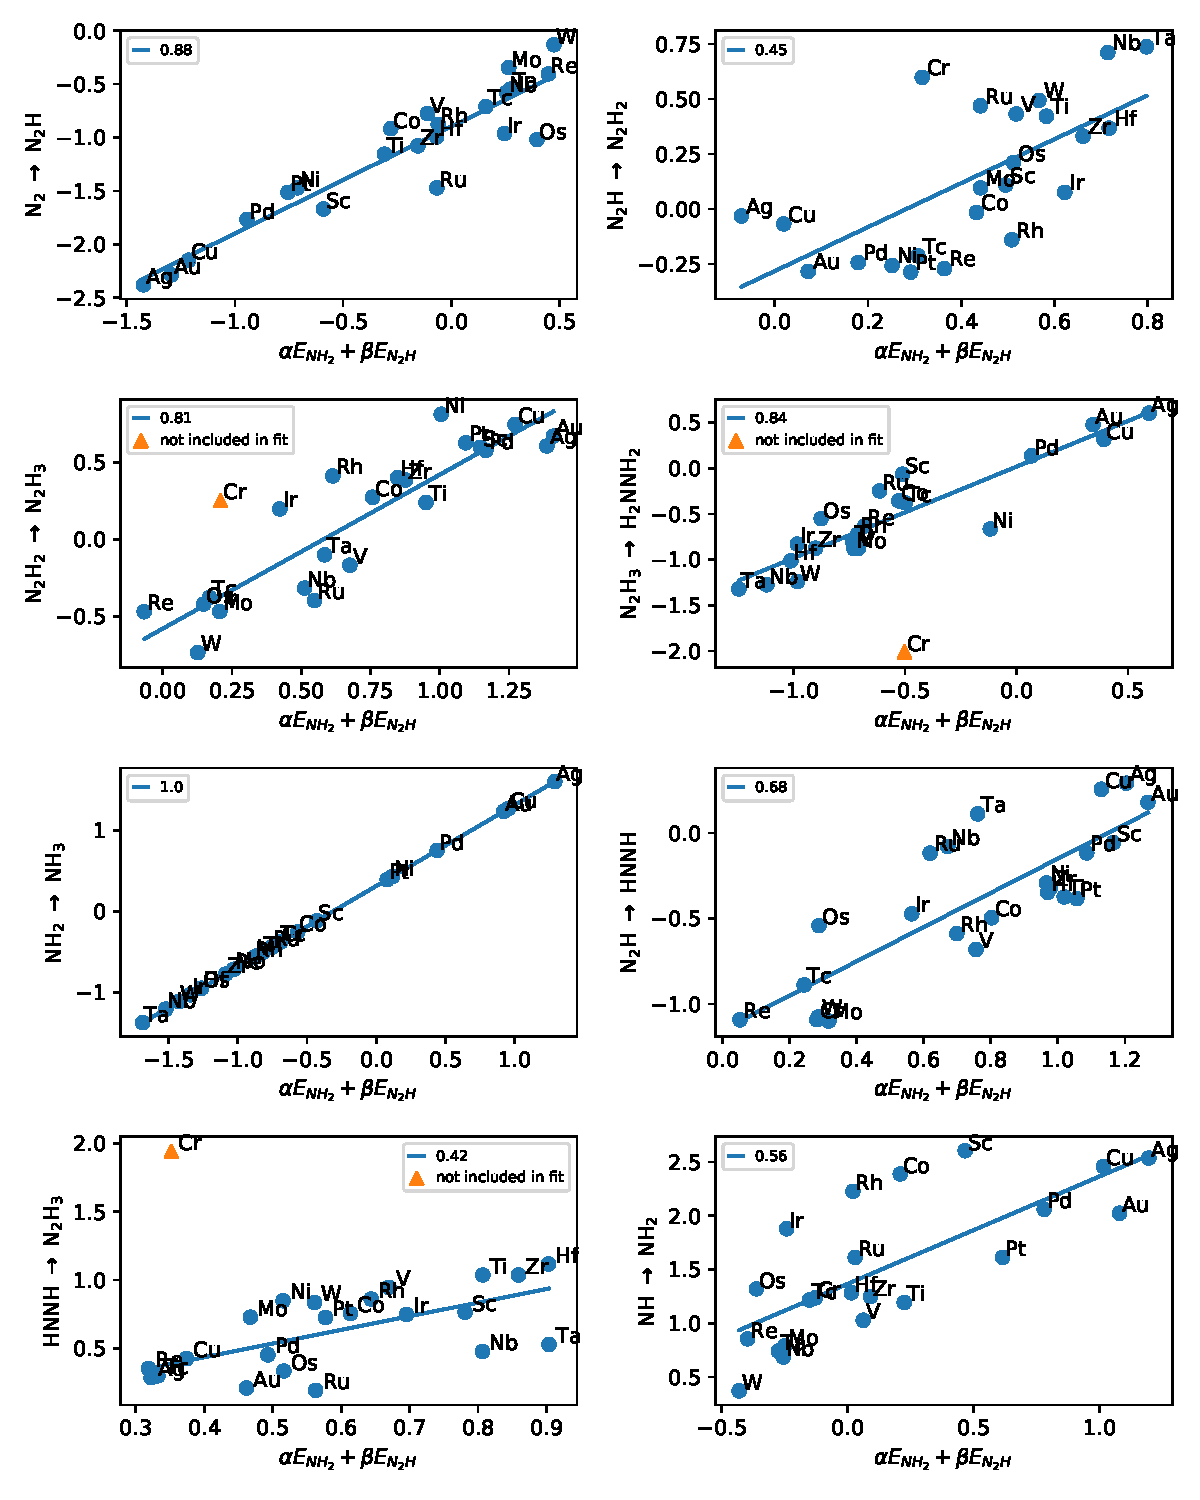
\includegraphics[width=0.8\linewidth]{Images/scaling_reactions.pdf}
\caption{The calculated scaling relations between the binding energies of various species and the binding energies of N$_2$H and NH$_2$ on 2+ dopant sites}
\end{figure}

\begin{figure}
\centering
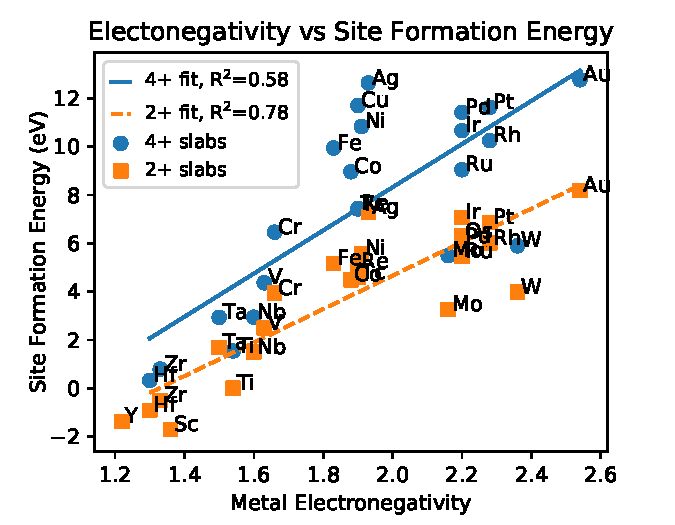
\includegraphics[width=0.8\linewidth]{Images/electronegativity_vs_formation.pdf}
\caption{Electronegativity vs formation energy of 2+ dopant site}
\end{figure}

\begin{figure}
\centering
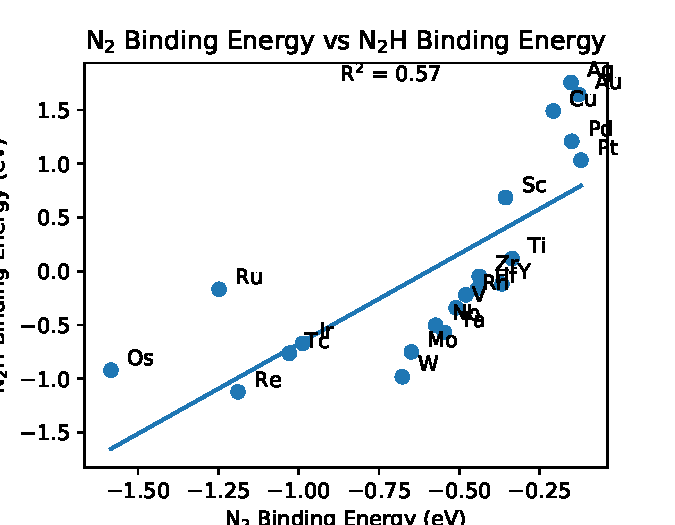
\includegraphics[width=0.8\linewidth]{Images/N2_vs_N2H.pdf}
\caption{The binding energy of N$_2$ vs N$_2$H}
\end{figure}

\begin{figure}
\centering
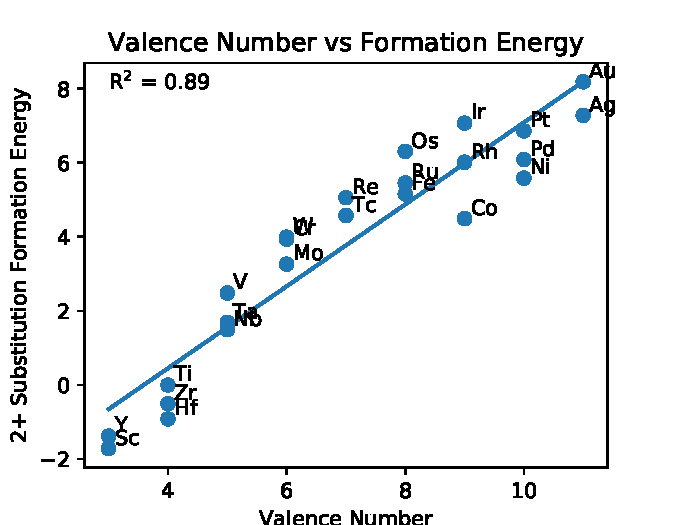
\includegraphics[width=0.8\linewidth]{Images/Valence_vs_formation_energy.pdf}
\caption{Valence number vs formation energy of 2+ dopant site}
\end{figure}

\begin{figure}
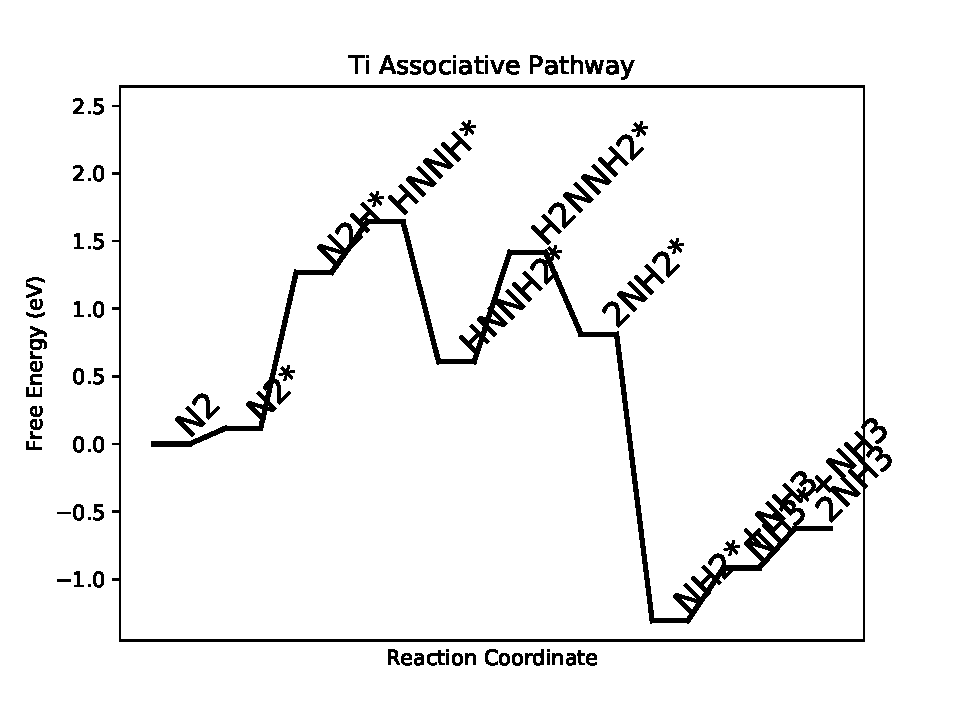
\includegraphics[width=0.8\linewidth]{data/plots/Ti_associative.pdf}
\end{figure}

\begin{figure}
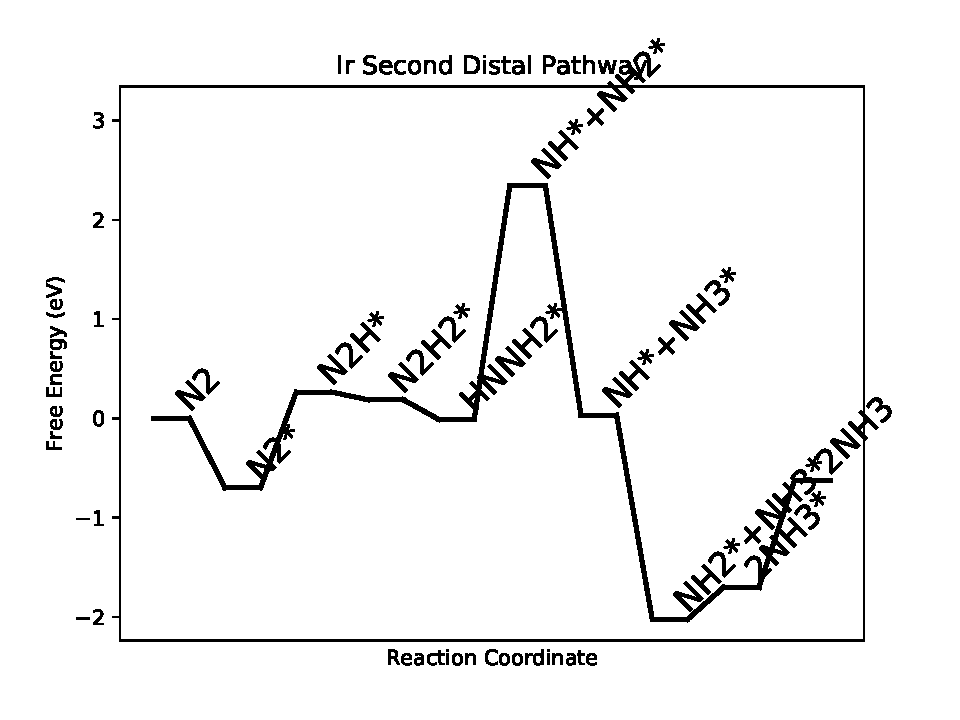
\includegraphics[width=0.8\linewidth]{data/plots/Ir_distal_2.pdf}
\end{figure}

\begin{figure}
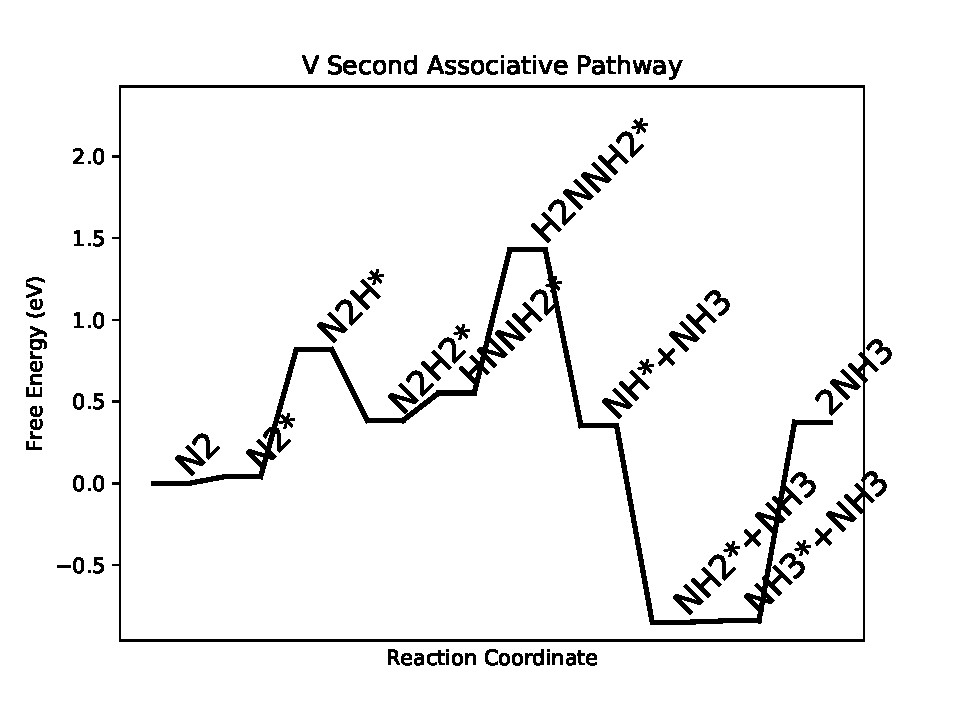
\includegraphics[width=0.8\linewidth]{data/plots/V_associative_2.pdf}
\end{figure}

\begin{figure}
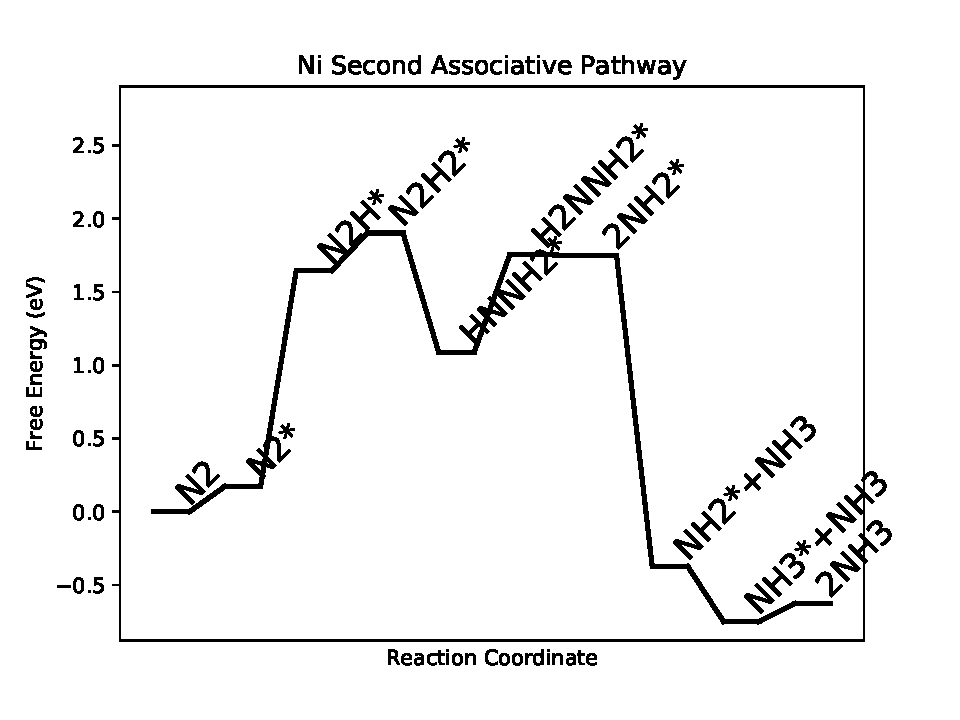
\includegraphics[width=0.8\linewidth]{data/plots/Ni_associative_2.pdf}
\end{figure}

\begin{figure}
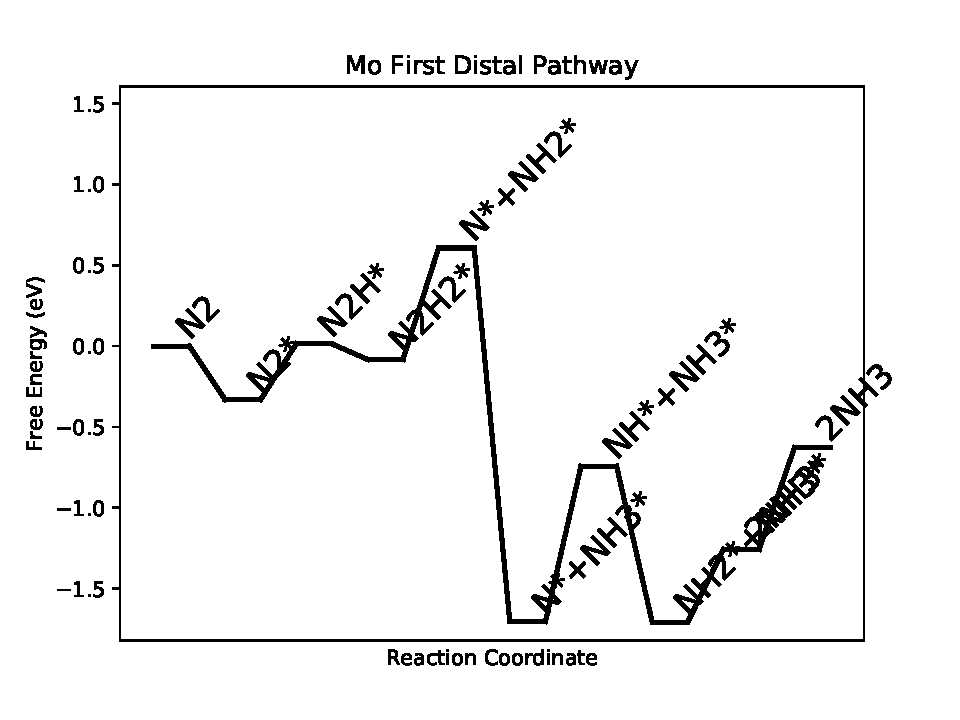
\includegraphics[width=0.8\linewidth]{data/plots/Mo_distal_1.pdf}
\end{figure}

\begin{figure}
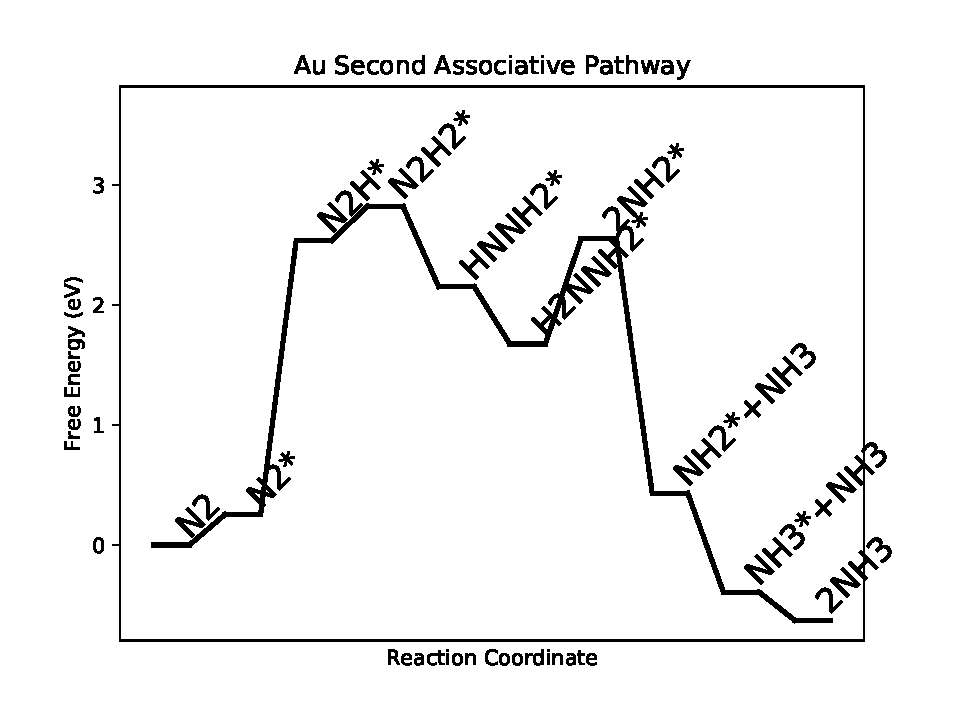
\includegraphics[width=0.8\linewidth]{data/plots/Au_associative_2.pdf}
\end{figure}

\begin{figure}
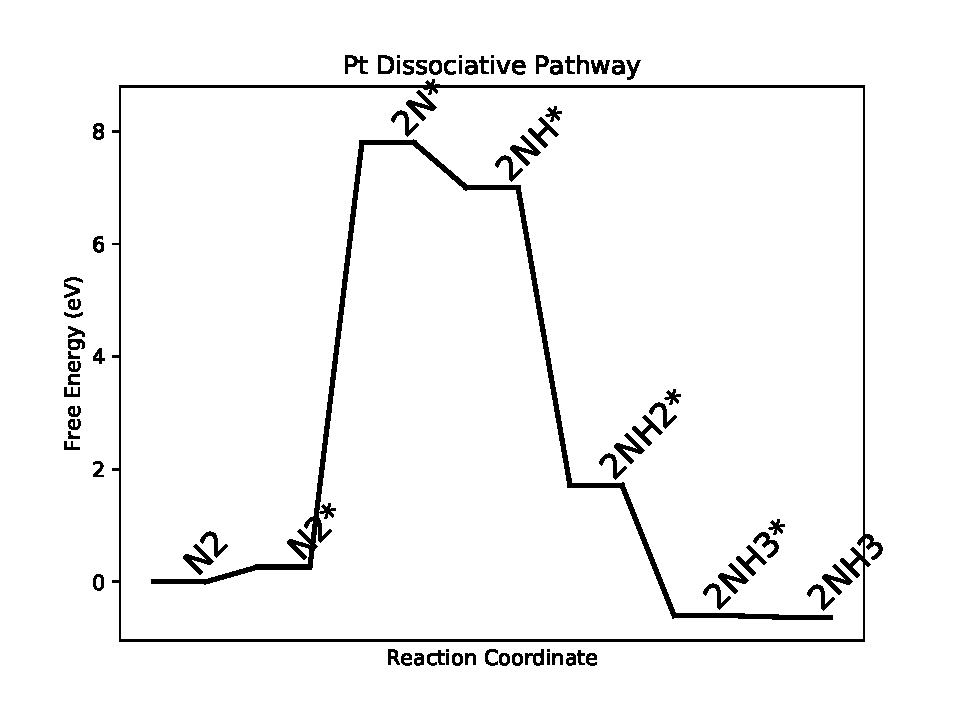
\includegraphics[width=0.8\linewidth]{data/plots/Pt_dissociative.pdf}
\end{figure}

\begin{figure}
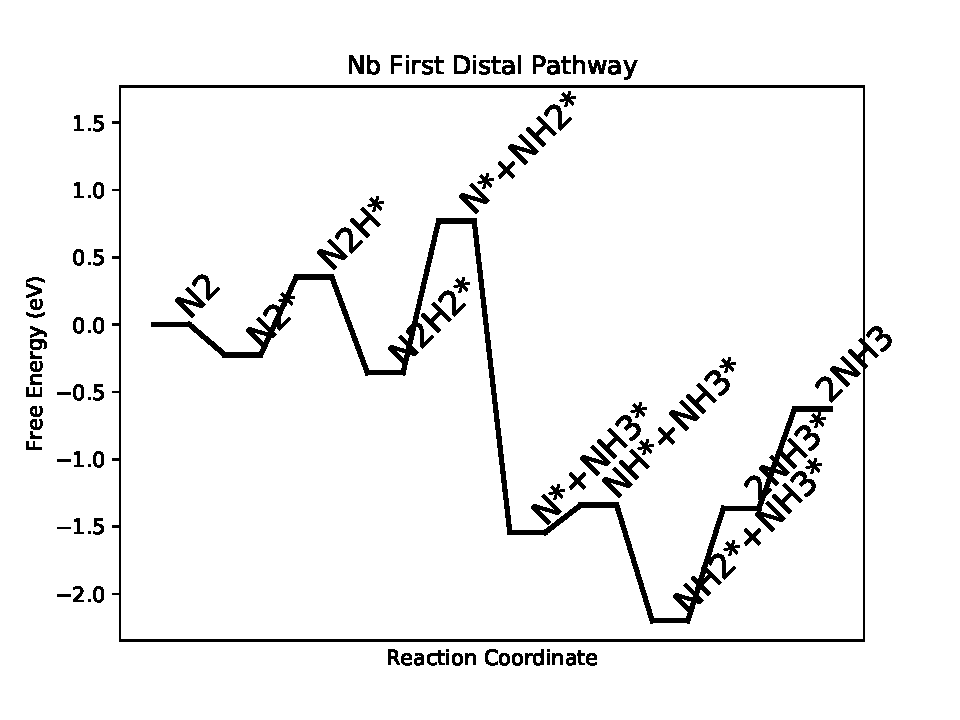
\includegraphics[width=0.8\linewidth]{data/plots/Nb_distal_1.pdf}
\end{figure}

\begin{figure}
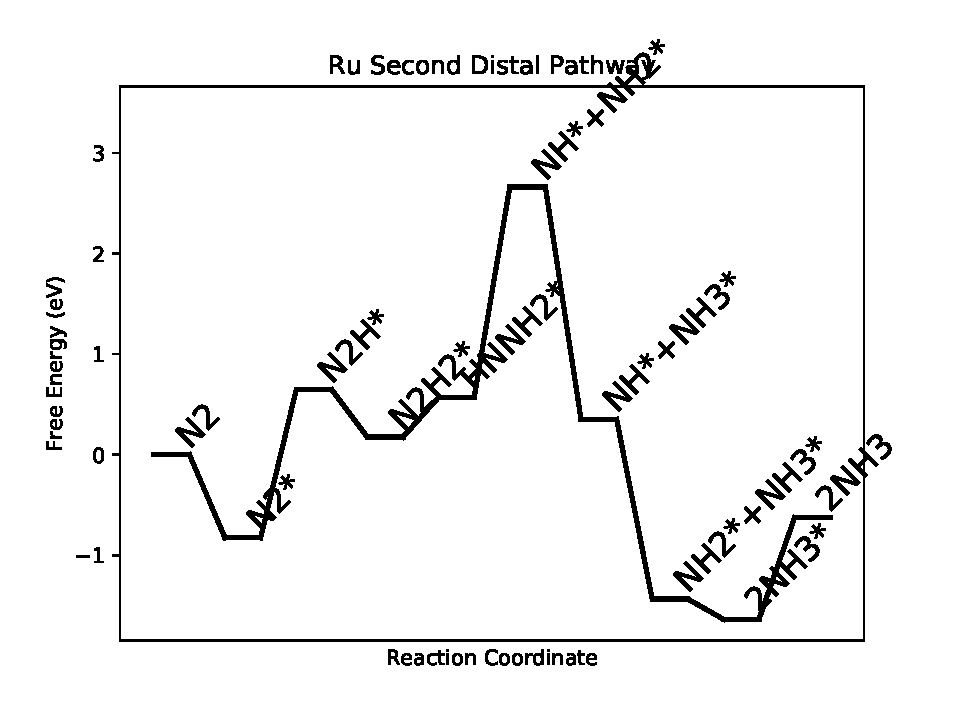
\includegraphics[width=0.8\linewidth]{data/plots/Ru_distal_2.pdf}
\end{figure}

\begin{figure}
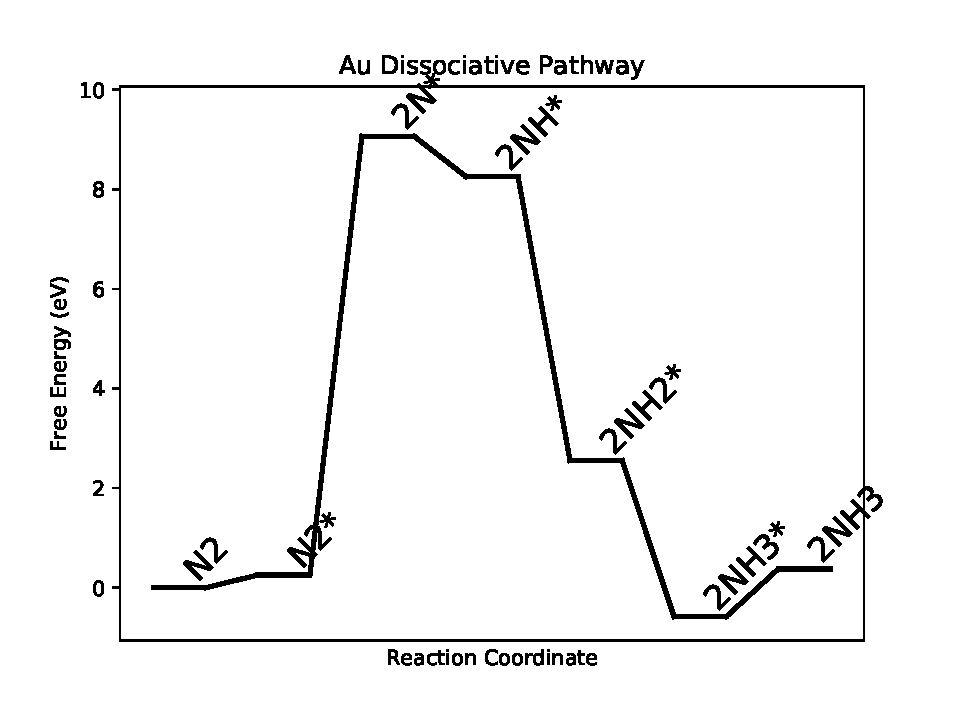
\includegraphics[width=0.8\linewidth]{data/plots/Au_dissociative.pdf}
\end{figure}

\begin{figure}
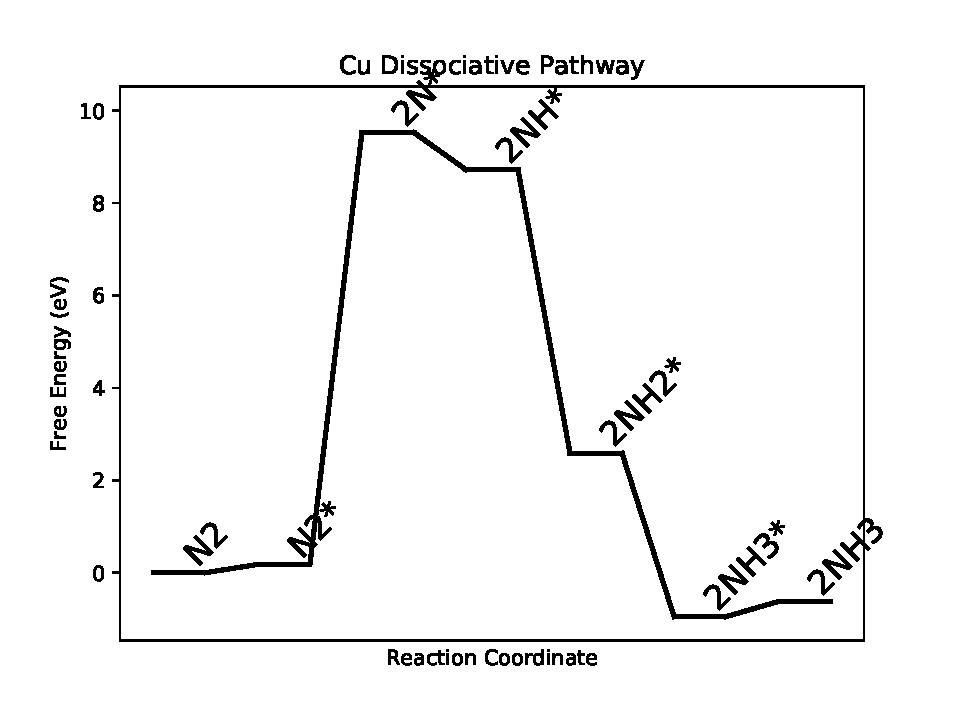
\includegraphics[width=0.8\linewidth]{data/plots/Cu_dissociative.pdf}
\end{figure}

\begin{figure}
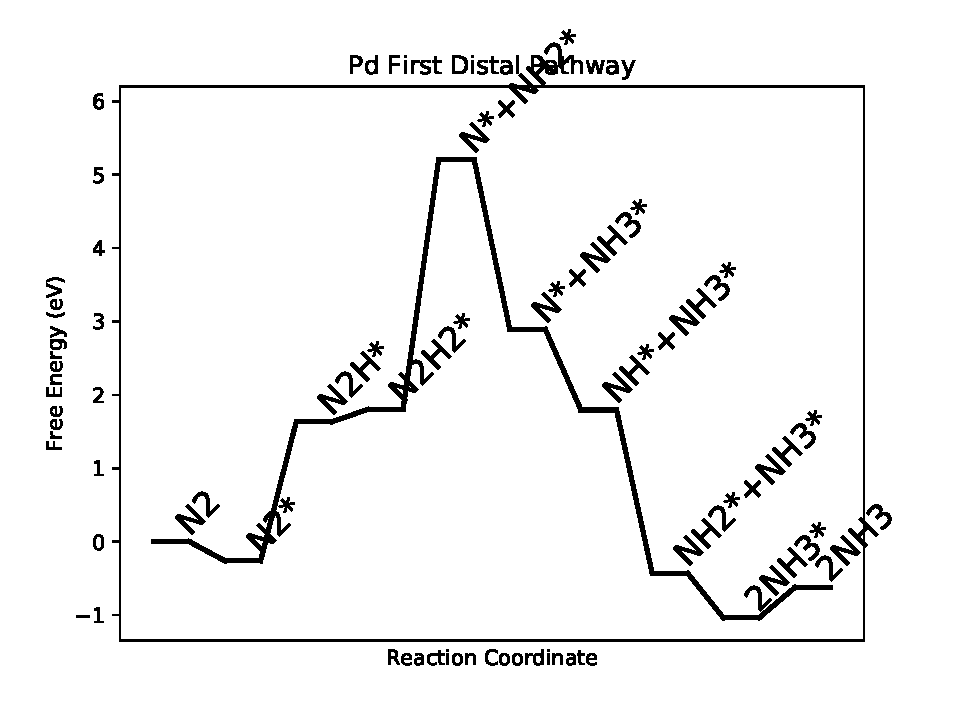
\includegraphics[width=0.8\linewidth]{data/plots/Pd_distal_1.pdf}
\end{figure}

\begin{figure}
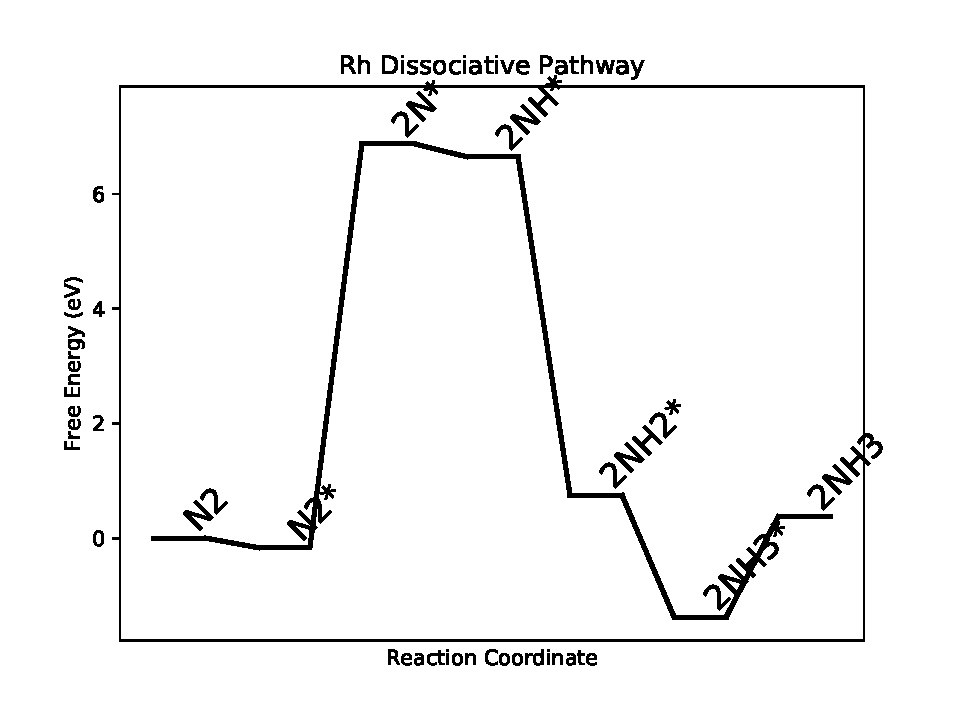
\includegraphics[width=0.8\linewidth]{data/plots/Rh_dissociative.pdf}
\end{figure}

\begin{figure}
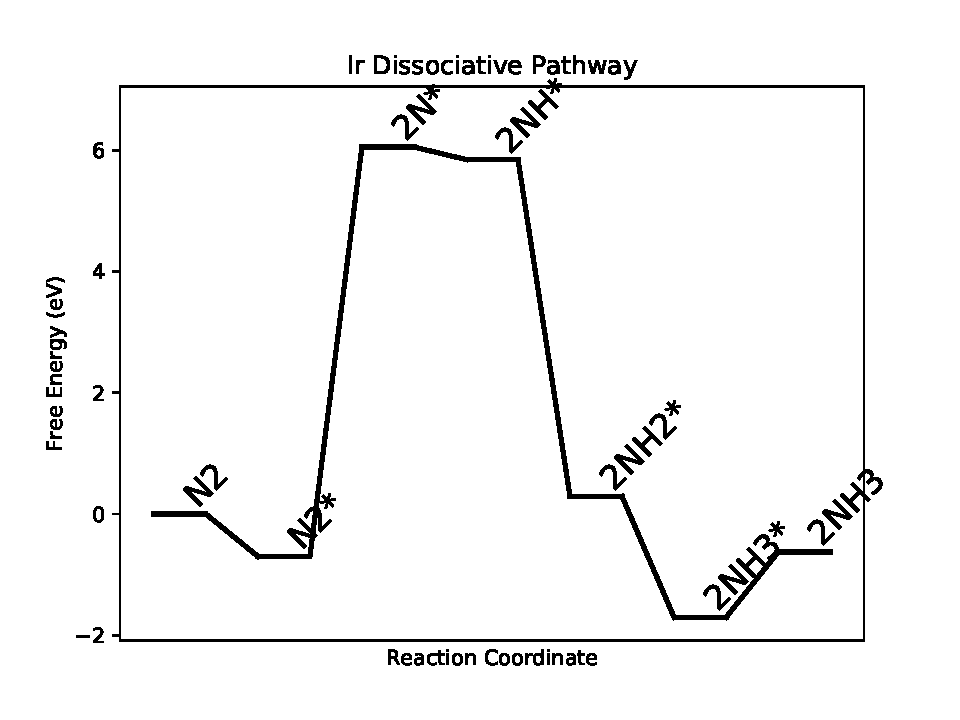
\includegraphics[width=0.8\linewidth]{data/plots/Ir_dissociative.pdf}
\end{figure}

\begin{figure}
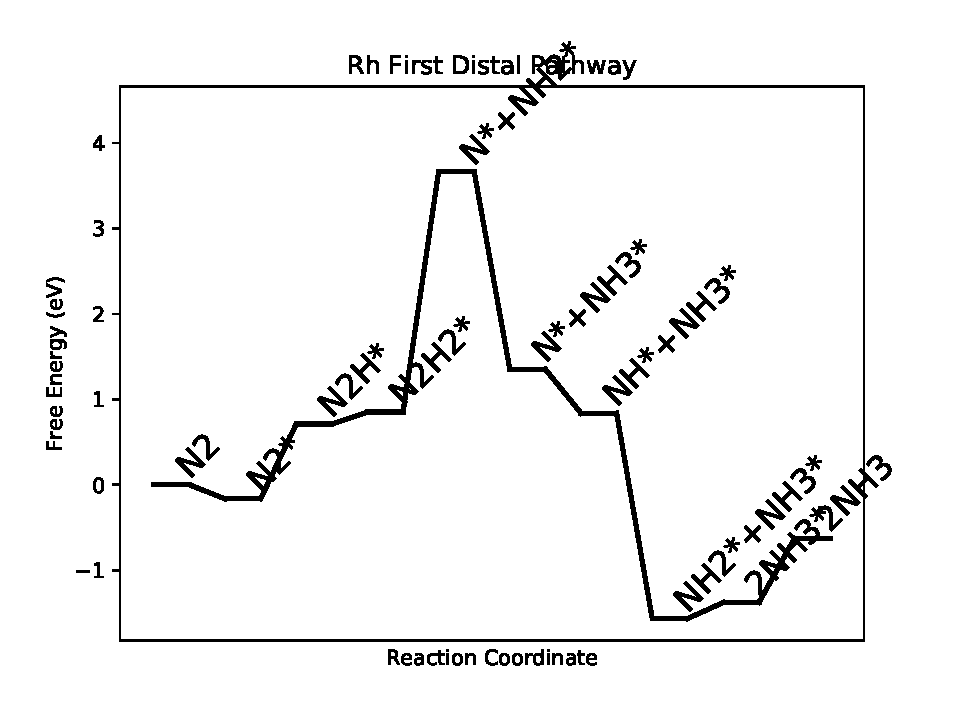
\includegraphics[width=0.8\linewidth]{data/plots/Rh_distal_1.pdf}
\end{figure}

\begin{figure}
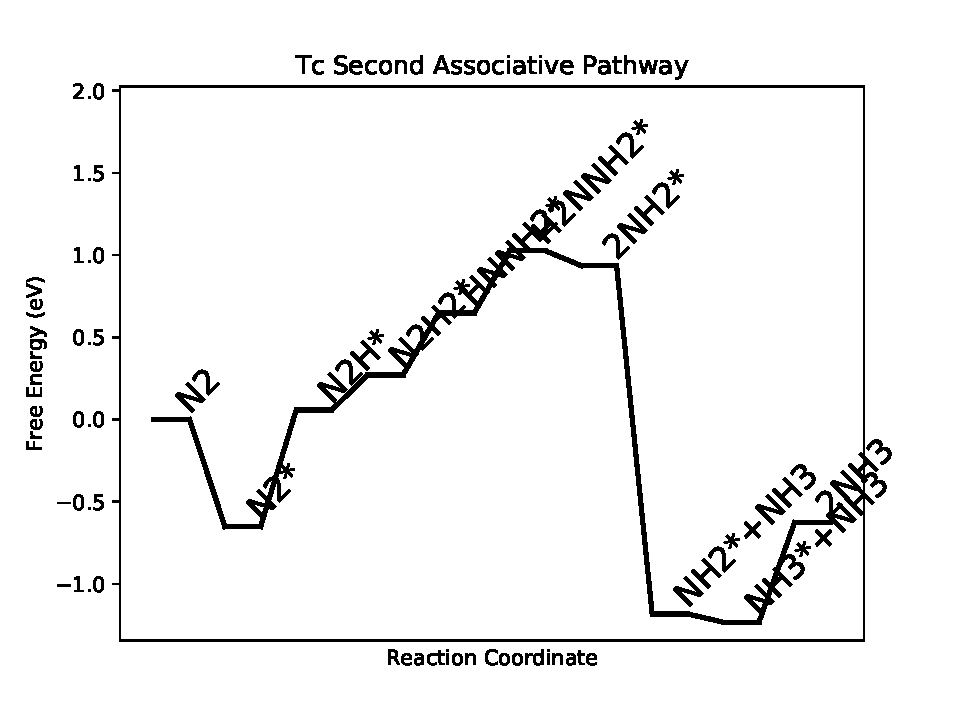
\includegraphics[width=0.8\linewidth]{data/plots/Tc_associative_2.pdf}
\end{figure}

\begin{figure}
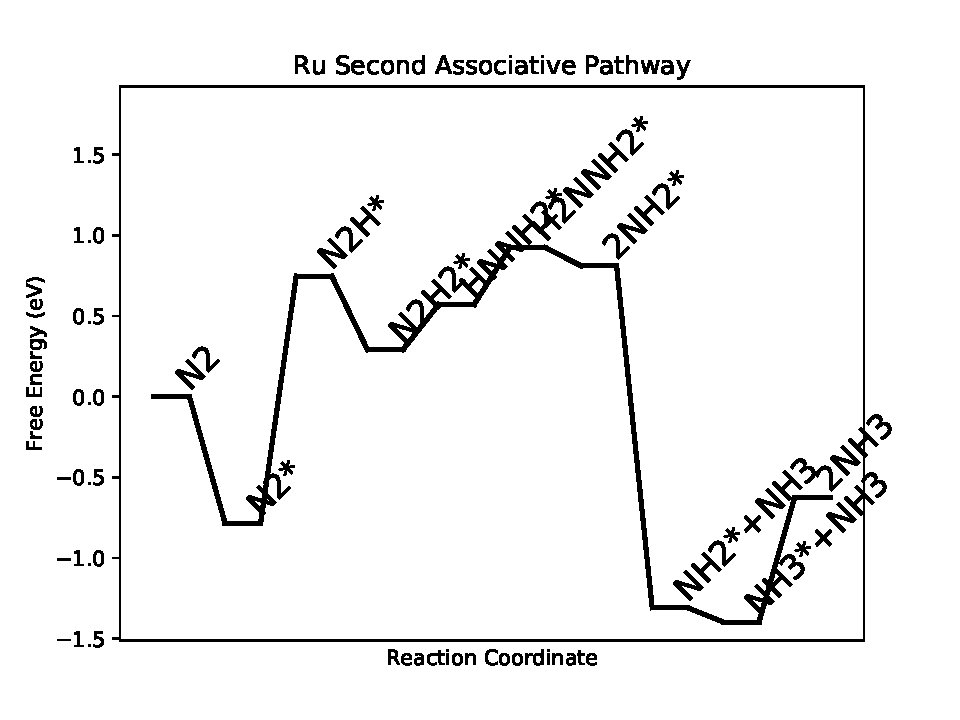
\includegraphics[width=0.8\linewidth]{data/plots/Ru_associative_2.pdf}
\end{figure}

\begin{figure}
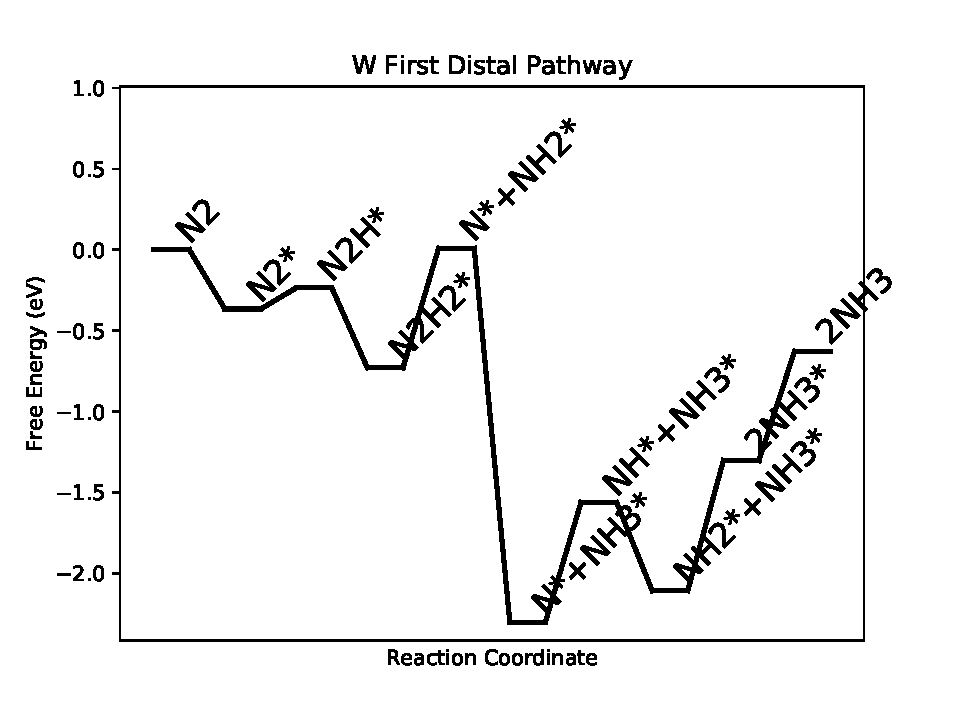
\includegraphics[width=0.8\linewidth]{data/plots/W_distal_1.pdf}
\end{figure}

\begin{figure}
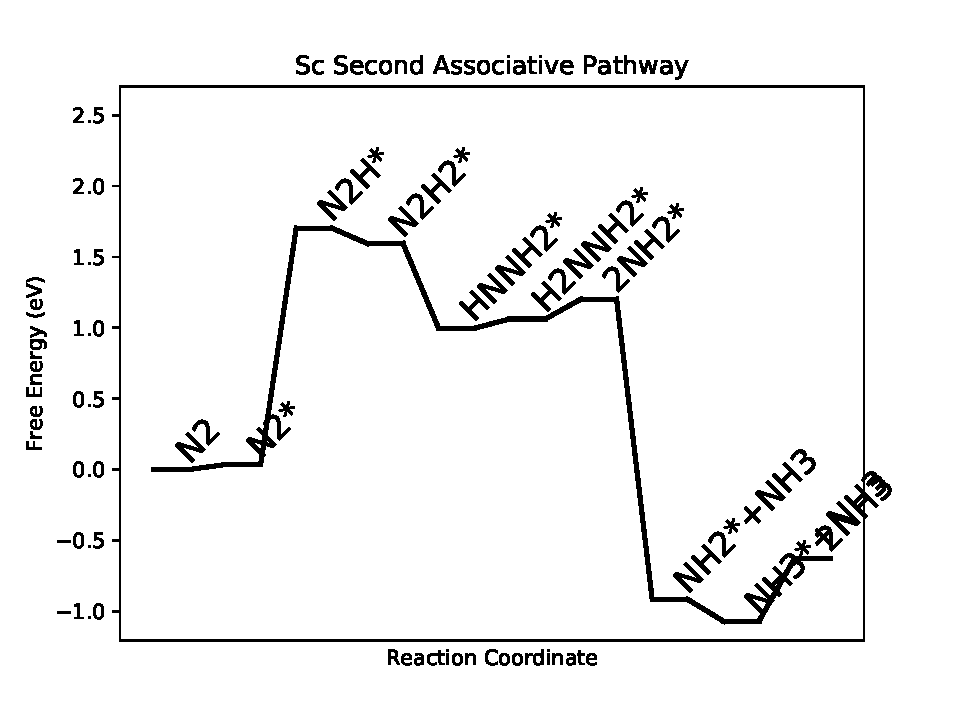
\includegraphics[width=0.8\linewidth]{data/plots/Sc_associative_2.pdf}
\end{figure}

\begin{figure}
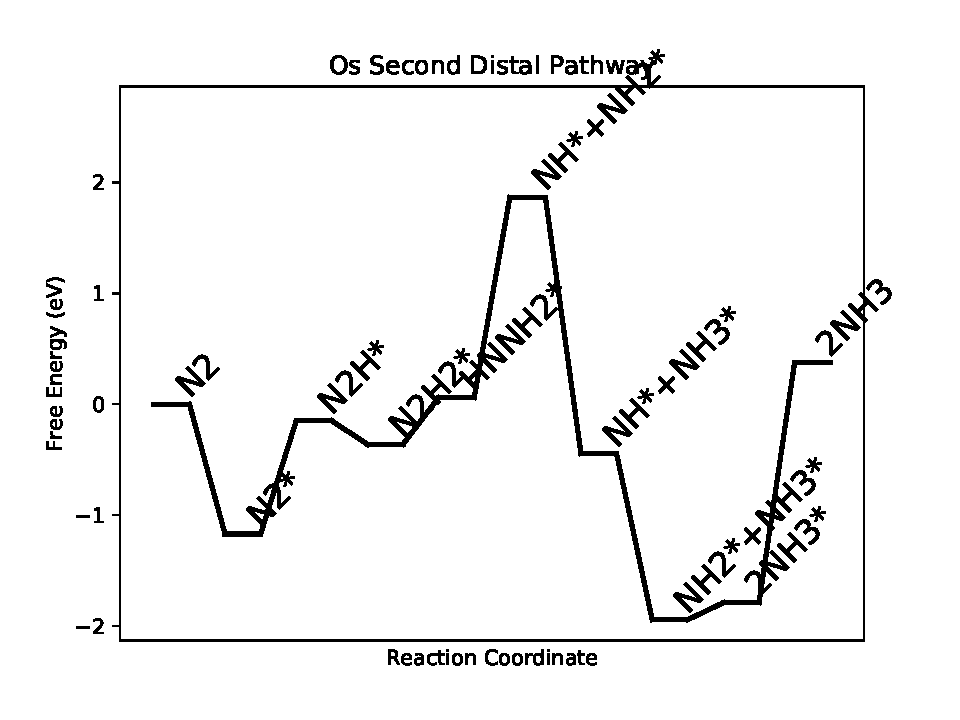
\includegraphics[width=0.8\linewidth]{data/plots/Os_distal_2.pdf}
\end{figure}

\begin{figure}
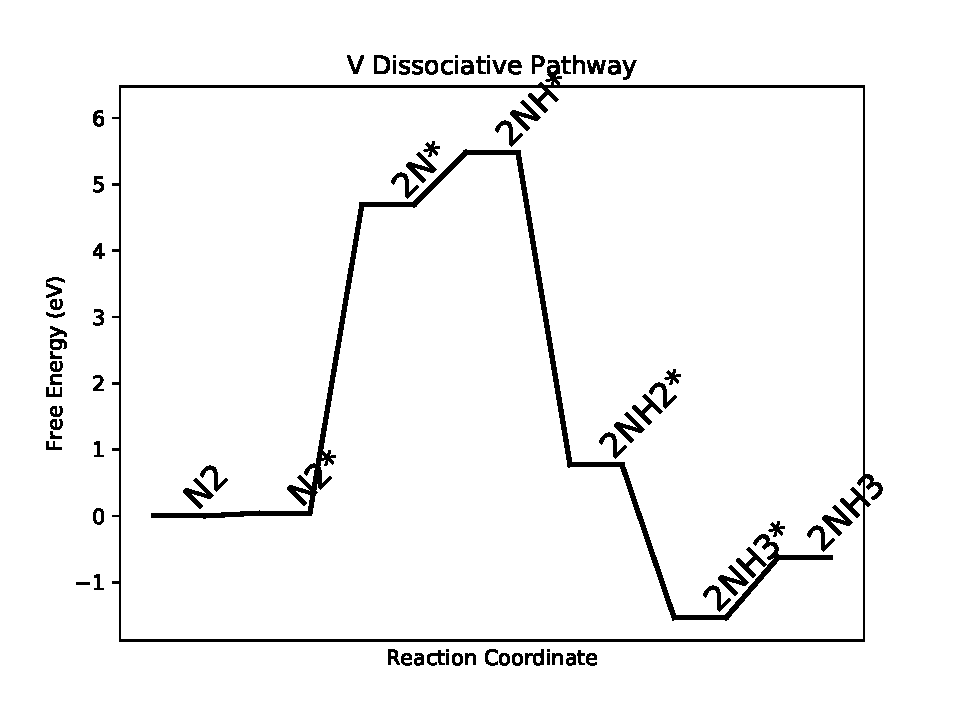
\includegraphics[width=0.8\linewidth]{data/plots/V_dissociative.pdf}
\end{figure}

\begin{figure}
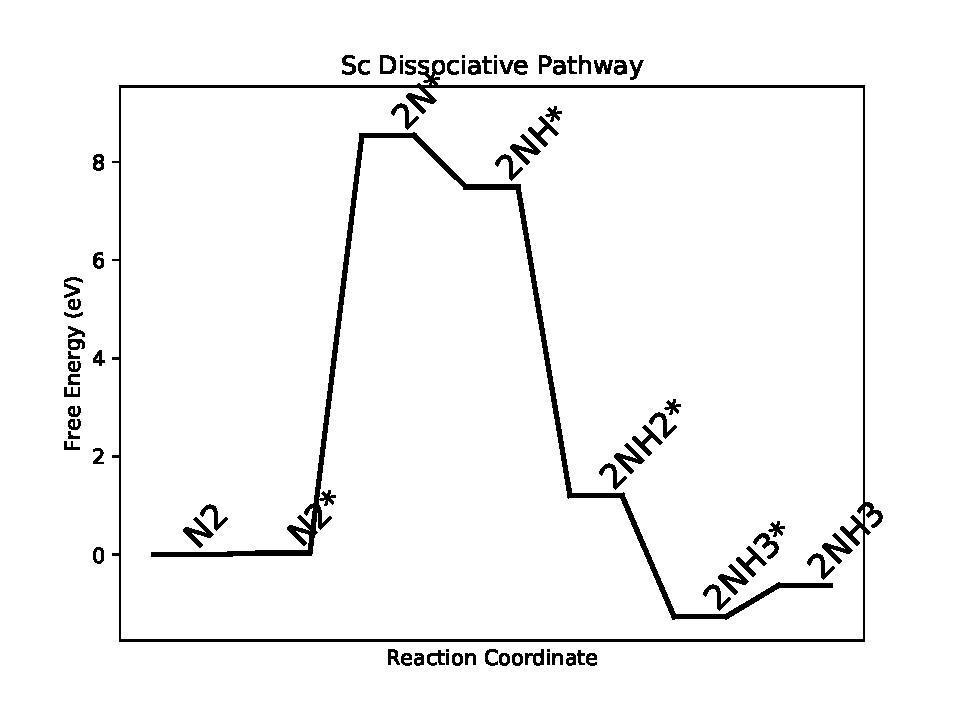
\includegraphics[width=0.8\linewidth]{data/plots/Sc_dissociative.pdf}
\end{figure}

\begin{figure}
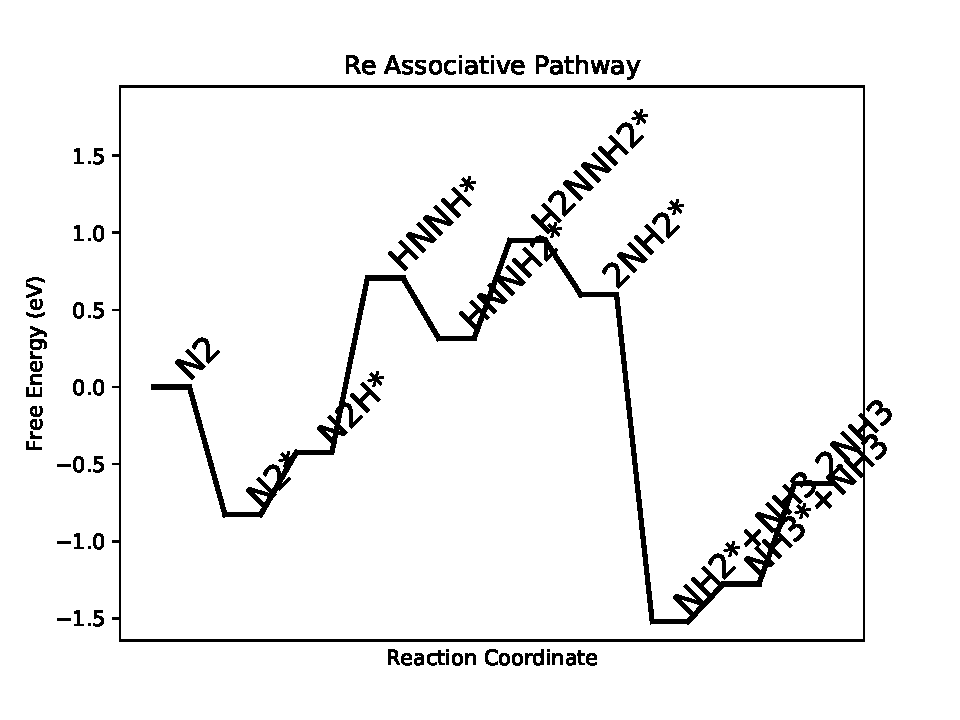
\includegraphics[width=0.8\linewidth]{data/plots/Re_associative.pdf}
\end{figure}

\begin{figure}
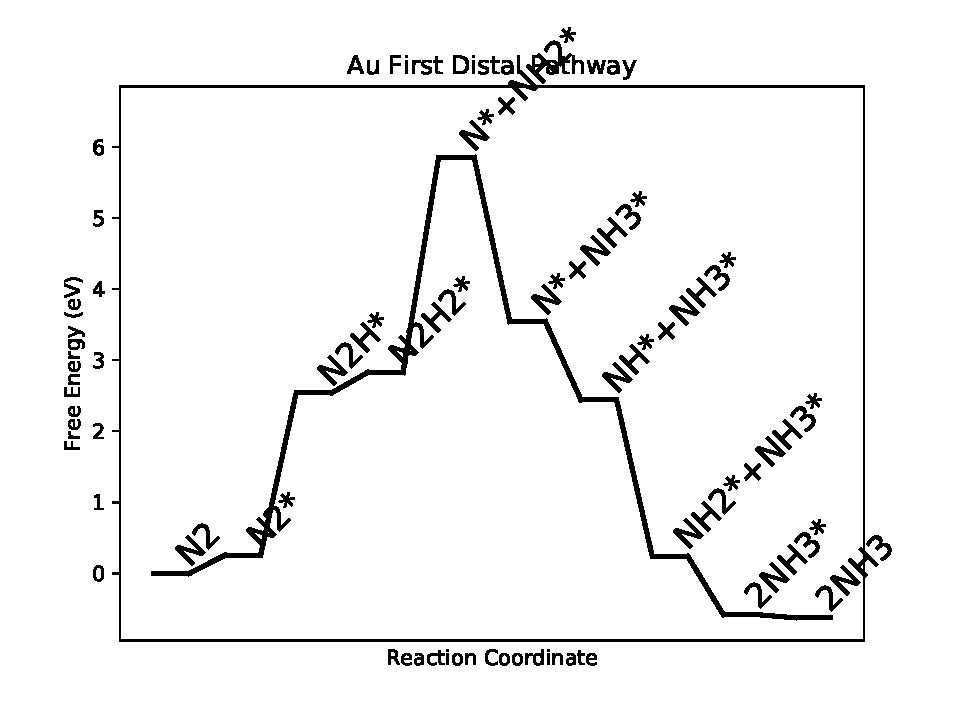
\includegraphics[width=0.8\linewidth]{data/plots/Au_distal_1.pdf}
\end{figure}

\begin{figure}
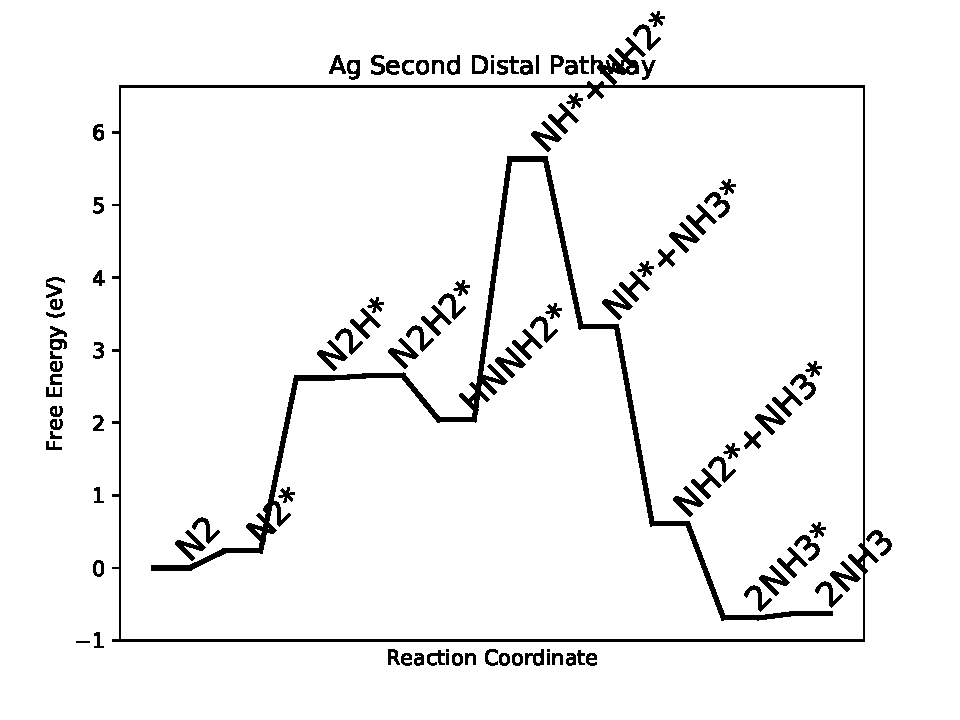
\includegraphics[width=0.8\linewidth]{data/plots/Ag_distal_2.pdf}
\end{figure}

\begin{figure}
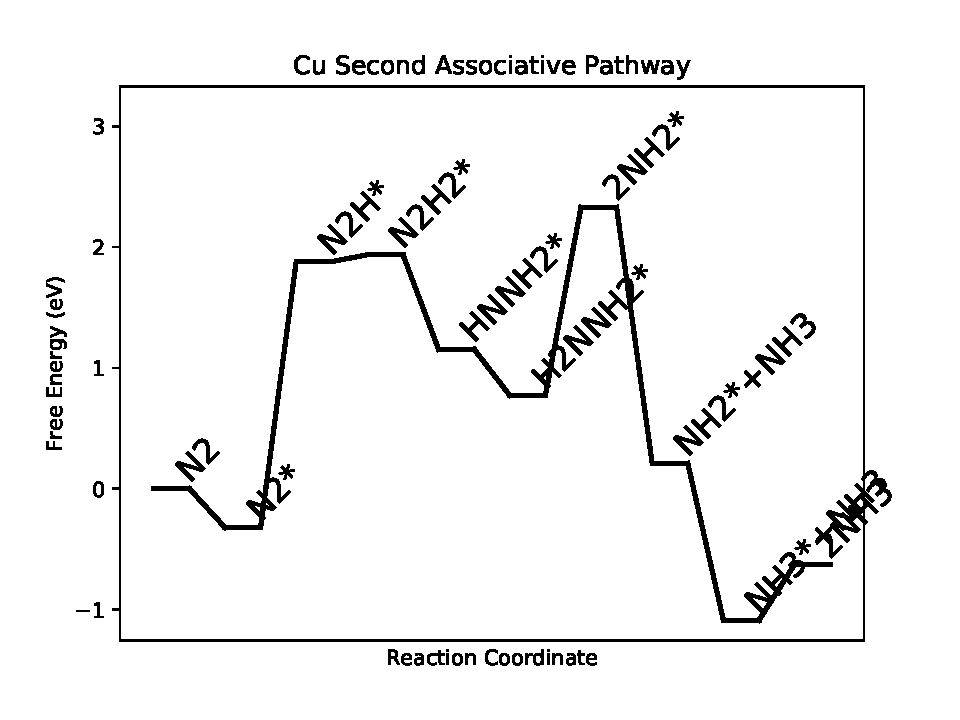
\includegraphics[width=0.8\linewidth]{data/plots/Cu_associative_2.pdf}
\end{figure}

\begin{figure}
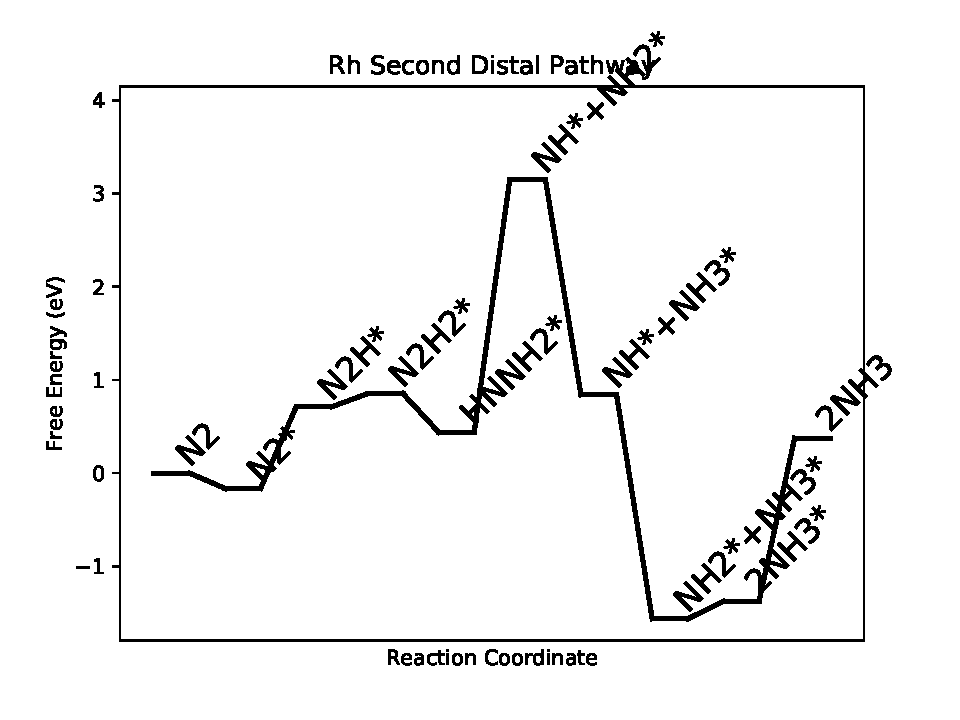
\includegraphics[width=0.8\linewidth]{data/plots/Rh_distal_2.pdf}
\end{figure}

\begin{figure}
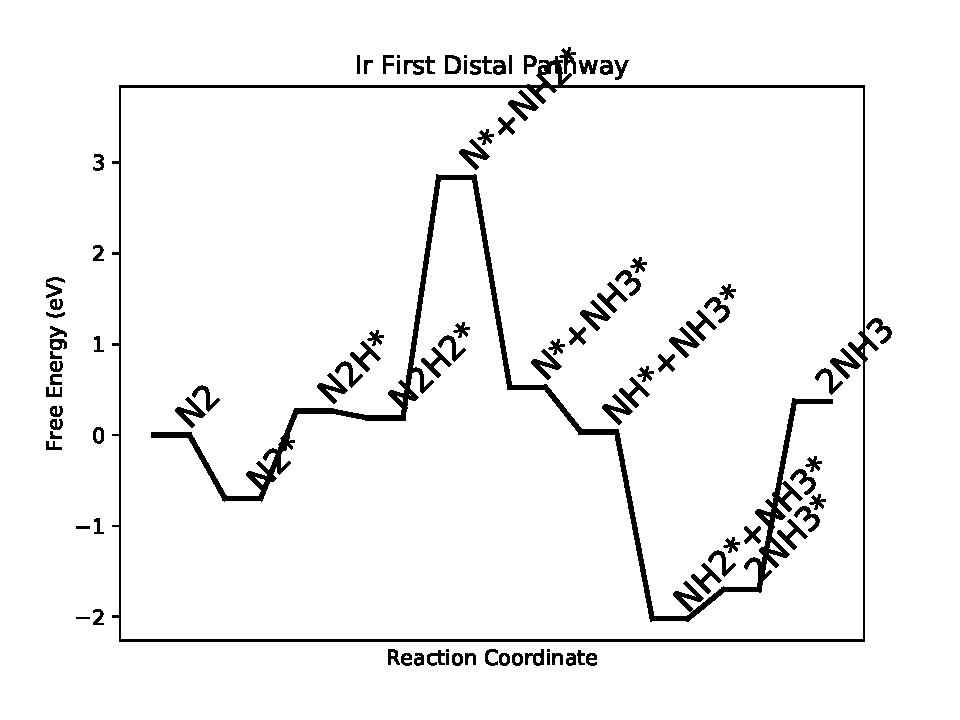
\includegraphics[width=0.8\linewidth]{data/plots/Ir_distal_1.pdf}
\end{figure}

\begin{figure}
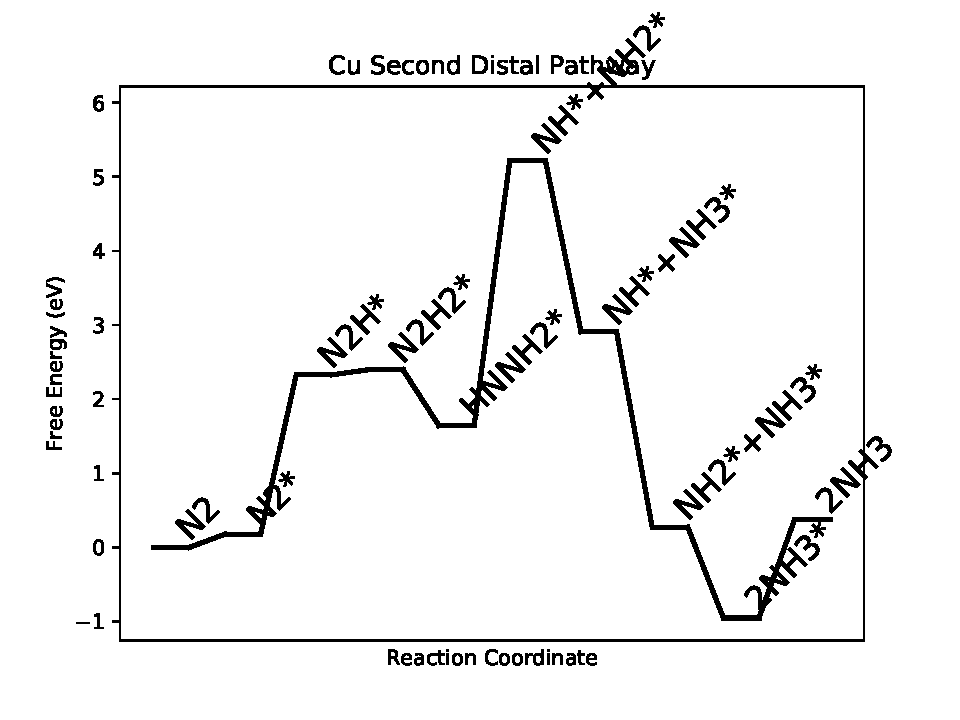
\includegraphics[width=0.8\linewidth]{data/plots/Cu_distal_2.pdf}
\end{figure}

\begin{figure}
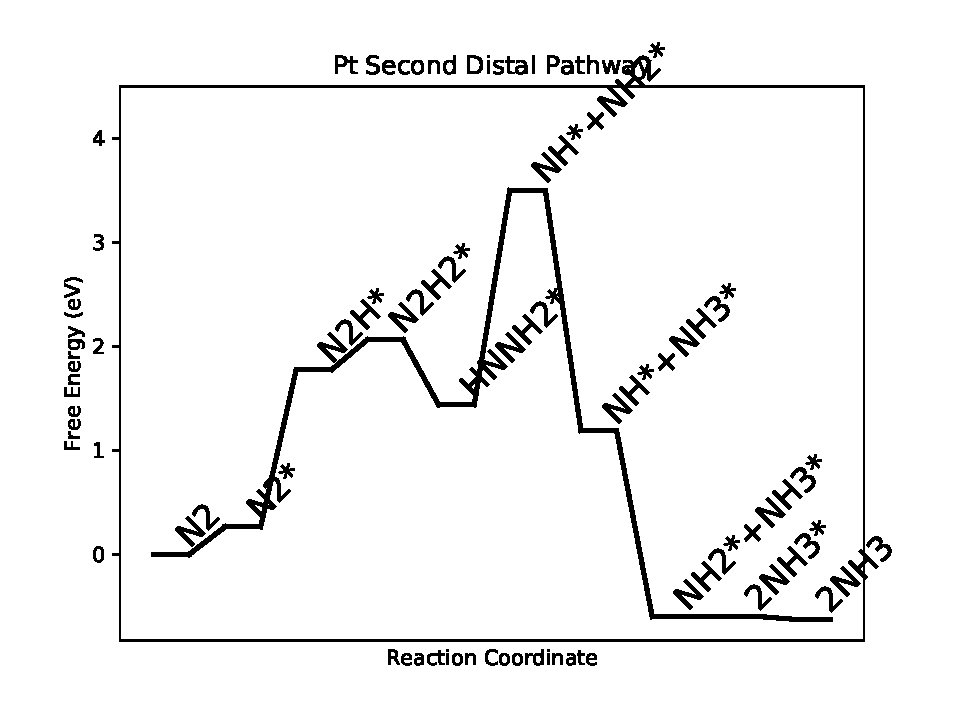
\includegraphics[width=0.8\linewidth]{data/plots/Pt_distal_2.pdf}
\end{figure}

\begin{figure}
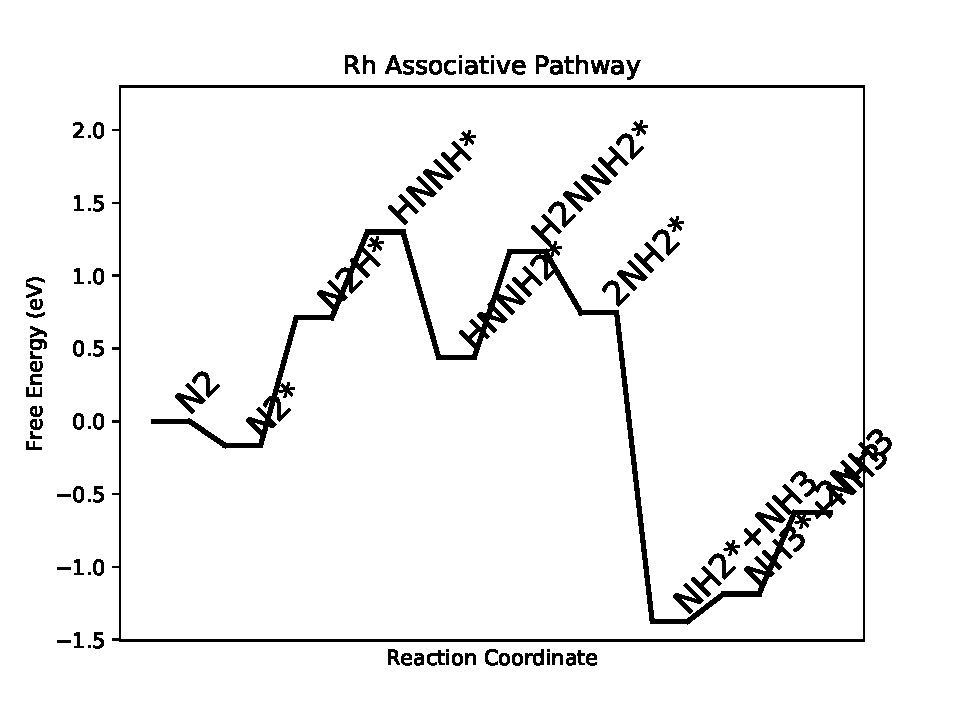
\includegraphics[width=0.8\linewidth]{data/plots/Rh_associative.pdf}
\end{figure}

\begin{figure}
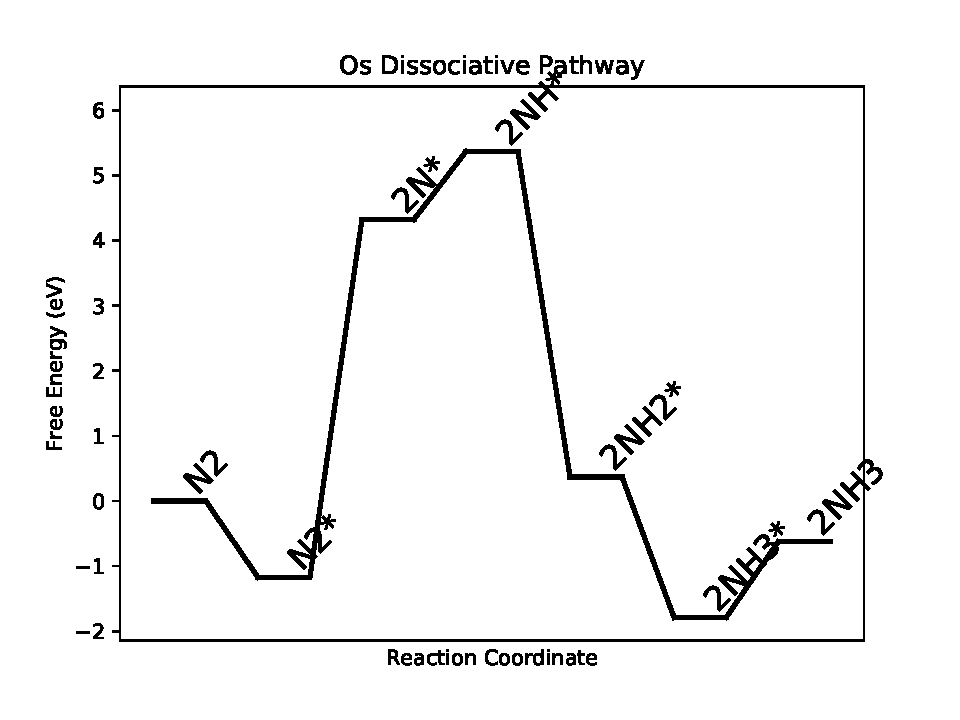
\includegraphics[width=0.8\linewidth]{data/plots/Os_dissociative.pdf}
\end{figure}

\begin{figure}
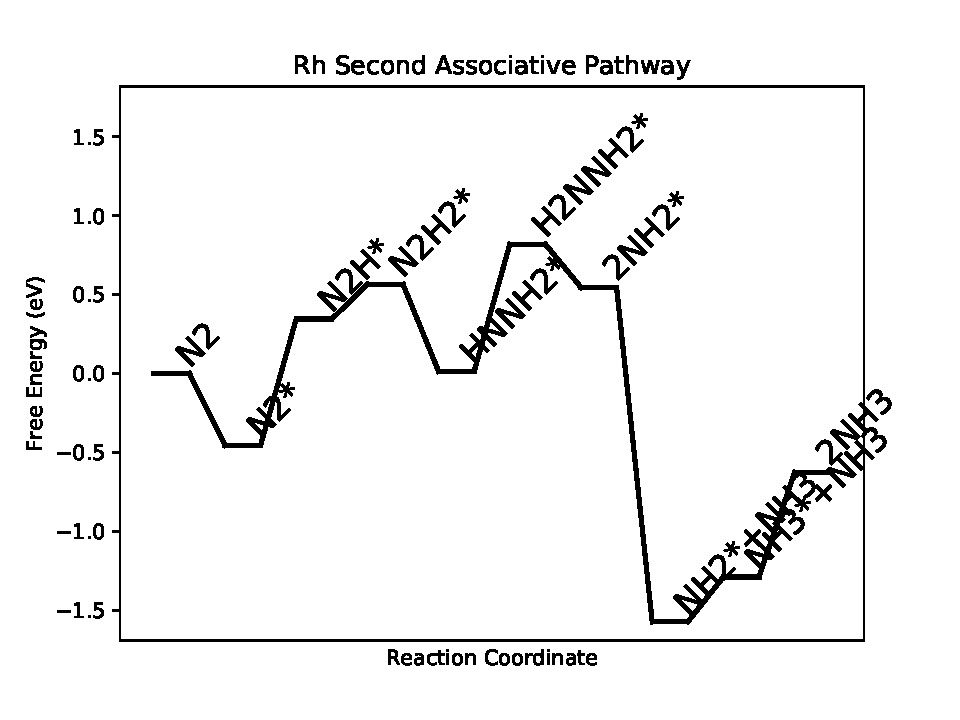
\includegraphics[width=0.8\linewidth]{data/plots/Rh_associative_2.pdf}
\end{figure}

\begin{figure}
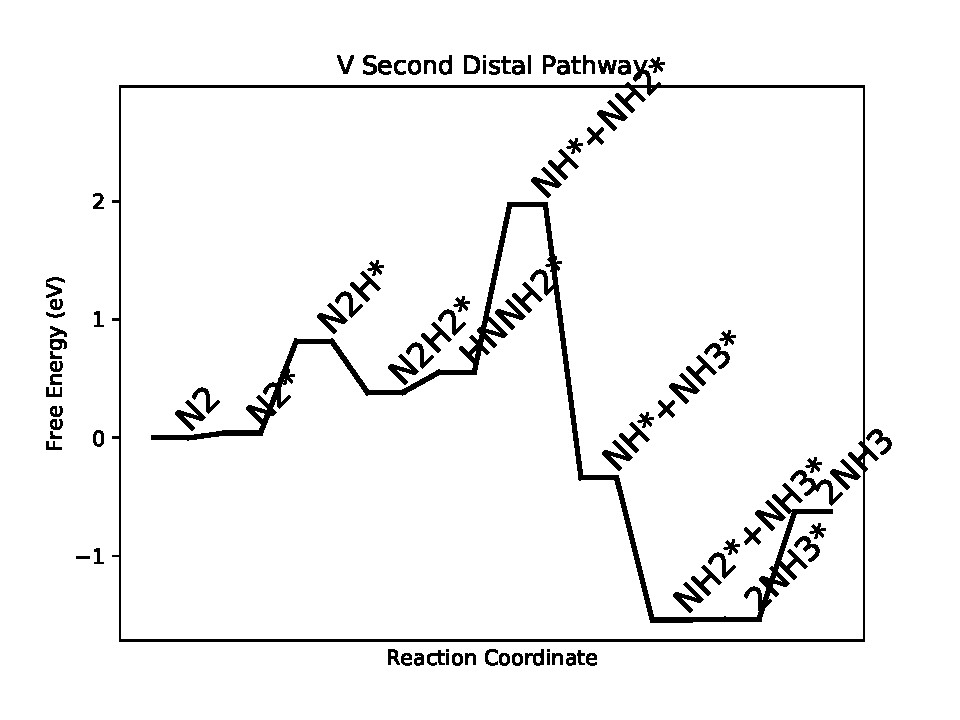
\includegraphics[width=0.8\linewidth]{data/plots/V_distal_2.pdf}
\end{figure}

\begin{figure}
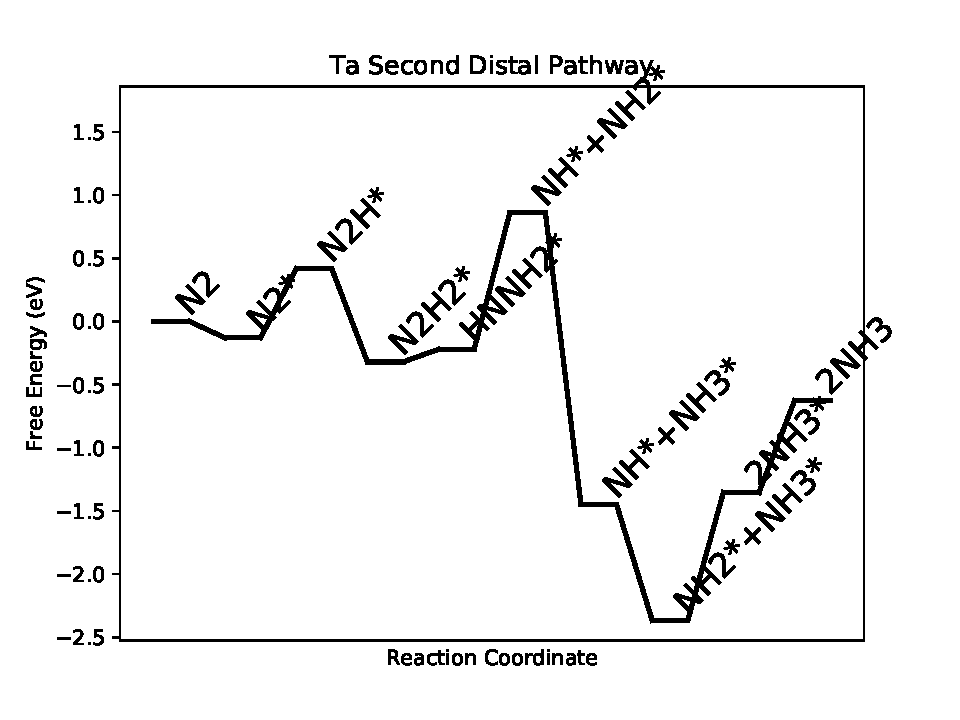
\includegraphics[width=0.8\linewidth]{data/plots/Ta_distal_2.pdf}
\end{figure}

\begin{figure}
\includegraphics[width=0.8\linewidth]{data/plots/Co_distal_1.pdf}
\end{figure}

\begin{figure}
\includegraphics[width=0.8\linewidth]{data/plots/Ru_dissociative.pdf}
\end{figure}

\begin{figure}
\includegraphics[width=0.8\linewidth]{data/plots/W_dissociative.pdf}
\end{figure}

\begin{figure}
\includegraphics[width=0.8\linewidth]{data/plots/Tc_dissociative.pdf}
\end{figure}

\begin{figure}
\includegraphics[width=0.8\linewidth]{data/plots/Tc_associative.pdf}
\end{figure}

\begin{figure}
\includegraphics[width=0.8\linewidth]{data/plots/Hf_associative.pdf}
\end{figure}

\begin{figure}
\includegraphics[width=0.8\linewidth]{data/plots/Os_associative_2.pdf}
\end{figure}

\begin{figure}
\includegraphics[width=0.8\linewidth]{data/plots/Ir_associative.pdf}
\end{figure}

\begin{figure}
\includegraphics[width=0.8\linewidth]{data/plots/Cu_distal_1.pdf}
\end{figure}

\begin{figure}
\includegraphics[width=0.8\linewidth]{data/plots/Re_dissociative.pdf}
\end{figure}

\begin{figure}
\includegraphics[width=0.8\linewidth]{data/plots/Ta_associative_2.pdf}
\end{figure}

\begin{figure}
\includegraphics[width=0.8\linewidth]{data/plots/Co_associative_2.pdf}
\end{figure}

\begin{figure}
\includegraphics[width=0.8\linewidth]{data/plots/Mo_associative_2.pdf}
\end{figure}

\begin{figure}
\includegraphics[width=0.8\linewidth]{data/plots/Nb_associative.pdf}
\end{figure}

\begin{figure}
\includegraphics[width=0.8\linewidth]{data/plots/Pd_associative.pdf}
\end{figure}

\begin{figure}
\includegraphics[width=0.8\linewidth]{data/plots/Tc_distal_2.pdf}
\end{figure}

\begin{figure}
\includegraphics[width=0.8\linewidth]{data/plots/Co_dissociative.pdf}
\end{figure}

\begin{figure}
\includegraphics[width=0.8\linewidth]{data/plots/Mo_associative.pdf}
\end{figure}

\begin{figure}
\includegraphics[width=0.8\linewidth]{data/plots/Pd_distal_2.pdf}
\end{figure}

\begin{figure}
\includegraphics[width=0.8\linewidth]{data/plots/Nb_associative_2.pdf}
\end{figure}

\begin{figure}
\includegraphics[width=0.8\linewidth]{data/plots/W_associative.pdf}
\end{figure}

\begin{figure}
\includegraphics[width=0.8\linewidth]{data/plots/Ag_dissociative.pdf}
\end{figure}

\begin{figure}
\includegraphics[width=0.8\linewidth]{data/plots/Y_dissociative.pdf}
\end{figure}

\begin{figure}
\includegraphics[width=0.8\linewidth]{data/plots/Nb_dissociative.pdf}
\end{figure}

\begin{figure}
\includegraphics[width=0.8\linewidth]{data/plots/Sc_distal_1.pdf}
\end{figure}

\begin{figure}
\includegraphics[width=0.8\linewidth]{data/plots/Nb_distal_2.pdf}
\end{figure}

\begin{figure}
\includegraphics[width=0.8\linewidth]{data/plots/W_distal_2.pdf}
\end{figure}

\begin{figure}
\includegraphics[width=0.8\linewidth]{data/plots/Ta_dissociative.pdf}
\end{figure}

\begin{figure}
\includegraphics[width=0.8\linewidth]{data/plots/Tc_distal_1.pdf}
\end{figure}

\begin{figure}
\includegraphics[width=0.8\linewidth]{data/plots/Re_distal_1.pdf}
\end{figure}

\begin{figure}
\includegraphics[width=0.8\linewidth]{data/plots/Ti_associative_2.pdf}
\end{figure}

\begin{figure}
\includegraphics[width=0.8\linewidth]{data/plots/Ru_distal_1.pdf}
\end{figure}

\begin{figure}
\includegraphics[width=0.8\linewidth]{data/plots/V_associative.pdf}
\end{figure}

\begin{figure}
\includegraphics[width=0.8\linewidth]{data/plots/Ni_associative.pdf}
\end{figure}

\begin{figure}
\includegraphics[width=0.8\linewidth]{data/plots/Hf_associative_2.pdf}
\end{figure}

\begin{figure}
\includegraphics[width=0.8\linewidth]{data/plots/Re_associative_2.pdf}
\end{figure}

\begin{figure}
\includegraphics[width=0.8\linewidth]{data/plots/Ir_associative_2.pdf}
\end{figure}

\begin{figure}
\includegraphics[width=0.8\linewidth]{data/plots/Ag_associative_2.pdf}
\end{figure}

\begin{figure}
\includegraphics[width=0.8\linewidth]{data/plots/Hf_distal_2.pdf}
\end{figure}

\begin{figure}
\includegraphics[width=0.8\linewidth]{data/plots/Re_distal_2.pdf}
\end{figure}

\begin{figure}
\includegraphics[width=0.8\linewidth]{data/plots/Au_distal_2.pdf}
\end{figure}

\begin{figure}
\includegraphics[width=0.8\linewidth]{data/plots/Sc_associative.pdf}
\end{figure}

\begin{figure}
\includegraphics[width=0.8\linewidth]{data/plots/Ti_distal_2.pdf}
\end{figure}

\begin{figure}
\includegraphics[width=0.8\linewidth]{data/plots/Mo_dissociative.pdf}
\end{figure}

\begin{figure}
\includegraphics[width=0.8\linewidth]{data/plots/Zr_dissociative.pdf}
\end{figure}

\begin{figure}
\includegraphics[width=0.8\linewidth]{data/plots/Ru_associative.pdf}
\end{figure}

\begin{figure}
\includegraphics[width=0.8\linewidth]{data/plots/Ag_distal_1.pdf}
\end{figure}

\begin{figure}
\includegraphics[width=0.8\linewidth]{data/plots/Os_associative.pdf}
\end{figure}

\begin{figure}
\includegraphics[width=0.8\linewidth]{data/plots/Ag_associative.pdf}
\end{figure}

\begin{figure}
\includegraphics[width=0.8\linewidth]{data/plots/Co_distal_2.pdf}
\end{figure}

\begin{figure}
\includegraphics[width=0.8\linewidth]{data/plots/Ta_distal_1.pdf}
\end{figure}

\begin{figure}
\includegraphics[width=0.8\linewidth]{data/plots/Zr_distal_2.pdf}
\end{figure}

\begin{figure}
\includegraphics[width=0.8\linewidth]{data/plots/Ta_associative.pdf}
\end{figure}

\begin{figure}
\includegraphics[width=0.8\linewidth]{data/plots/Pt_distal_1.pdf}
\end{figure}

\begin{figure}
\includegraphics[width=0.8\linewidth]{data/plots/Cu_associative.pdf}
\end{figure}

\begin{figure}
\includegraphics[width=0.8\linewidth]{data/plots/Pd_associative_2.pdf}
\end{figure}

\begin{figure}
\includegraphics[width=0.8\linewidth]{data/plots/Pd_dissociative.pdf}
\end{figure}

\begin{figure}
\includegraphics[width=0.8\linewidth]{data/plots/Co_associative.pdf}
\end{figure}

\begin{figure}
\includegraphics[width=0.8\linewidth]{data/plots/Au_associative.pdf}
\end{figure}

\begin{figure}
\includegraphics[width=0.8\linewidth]{data/plots/V_distal_1.pdf}
\end{figure}

\begin{figure}
\includegraphics[width=0.8\linewidth]{data/plots/Ti_dissociative.pdf}
\end{figure}

\begin{figure}
\includegraphics[width=0.8\linewidth]{data/plots/Mo_distal_2.pdf}
\end{figure}

\begin{figure}
\includegraphics[width=0.8\linewidth]{data/plots/Sc_distal_2.pdf}
\end{figure}

\begin{figure}
\includegraphics[width=0.8\linewidth]{data/plots/Zr_associative_2.pdf}
\end{figure}

\begin{figure}
\includegraphics[width=0.8\linewidth]{data/plots/Zr_associative.pdf}
\end{figure}

\begin{figure}
\includegraphics[width=0.8\linewidth]{data/plots/Os_distal_1.pdf}
\end{figure}

\begin{figure}
\includegraphics[width=0.8\linewidth]{data/plots/Ti_distal_1.pdf}
\end{figure}

\begin{figure}
\includegraphics[width=0.8\linewidth]{data/plots/Hf_dissociative.pdf}
\end{figure}

\begin{figure}
\includegraphics[width=0.8\linewidth]{data/plots/W_associative_2.pdf}
\end{figure}

\begin{figure}
\includegraphics[width=0.8\linewidth]{data/plots/Zr_distal_1.pdf}
\end{figure}

\begin{figure}
\includegraphics[width=0.8\linewidth]{data/plots/Hf_distal_1.pdf}
\end{figure}


\end{document}
%One route to increasing reaction rates is the the inclusion of transition-metal dopants in TiO$_2$. Transition-metal dopants can increase rates via two distinct mechanisms: increasing the amount of photo-generated electrons that reach the surface by improving absorption and charge separation, or by altering the kinetics of the surface reaction.

